\documentclass[a4paper]{book}
\usepackage{makeidx}
\usepackage{graphicx}
\usepackage{multicol}
\usepackage{float}
\usepackage{listings}
\usepackage{color}
\usepackage{ifthen}
\usepackage[table]{xcolor}
\usepackage{textcomp}
\usepackage{alltt}
\usepackage{ifpdf}
\ifpdf
\usepackage[pdftex,
            pagebackref=true,
            colorlinks=true,
            linkcolor=blue,
            unicode
           ]{hyperref}
\else
\usepackage[ps2pdf,
            pagebackref=true,
            colorlinks=true,
            linkcolor=blue,
            unicode
           ]{hyperref}
\usepackage{pspicture}
\fi
\usepackage[utf8]{inputenc}
\usepackage{mathptmx}
\usepackage[scaled=.90]{helvet}
\usepackage{courier}
\usepackage{doxygen}
\lstset{language=C++,inputencoding=utf8,basicstyle=\footnotesize,breaklines=true,breakatwhitespace=true,tabsize=8,numbers=left }
\makeindex
\setcounter{tocdepth}{3}
\renewcommand{\footrulewidth}{0.4pt}
\begin{document}
\hypersetup{pageanchor=false}
\begin{titlepage}
\vspace*{7cm}
\begin{center}
{\Large Parse Utils \\[1ex]\large v0.1a }\\
\vspace*{1cm}
{\large Generated by Doxygen 1.7.3}\\
\vspace*{0.5cm}
{\small Fri Jun 22 2012 13:47:23}\\
\end{center}
\end{titlepage}
\clearemptydoublepage
\pagenumbering{roman}
\tableofcontents
\clearemptydoublepage
\pagenumbering{arabic}
\hypersetup{pageanchor=true}
\chapter{Class Index}
\section{Class Hierarchy}
This inheritance list is sorted roughly, but not completely, alphabetically\-:\begin{DoxyCompactList}
\item \contentsline{section}{A\-S\-T}{\pageref{class_a_s_t}}{}
\item \contentsline{section}{Exception}{\pageref{class_exception}}{}
\item \contentsline{section}{I\-Lexer}{\pageref{class_i_lexer}}{}
\begin{DoxyCompactList}
\item \contentsline{section}{L\-L\-N\-Lexer}{\pageref{class_l_l_n_lexer}}{}
\end{DoxyCompactList}
\item \contentsline{section}{I\-Marker}{\pageref{class_i_marker}}{}
\begin{DoxyCompactList}
\item \contentsline{section}{B\-T\-Parser}{\pageref{class_b_t_parser}}{}
\item \contentsline{section}{I\-Buffer}{\pageref{class_i_buffer}}{}
\end{DoxyCompactList}
\item \contentsline{section}{I\-Parser}{\pageref{class_i_parser}}{}
\begin{DoxyCompactList}
\item \contentsline{section}{B\-T\-Parser}{\pageref{class_b_t_parser}}{}
\end{DoxyCompactList}
\item \contentsline{section}{I\-Visitor}{\pageref{class_i_visitor}}{}
\begin{DoxyCompactList}
\item \contentsline{section}{A\-S\-T\-Printer}{\pageref{class_a_s_t_printer}}{}
\end{DoxyCompactList}
\item \contentsline{section}{Scope\-Stack}{\pageref{class_scope_stack}}{}
\item \contentsline{section}{Symbol}{\pageref{class_symbol}}{}
\item \contentsline{section}{Token}{\pageref{class_token}}{}
\end{DoxyCompactList}

\chapter{Class Index}
\section{Class List}
Here are the classes, structs, unions and interfaces with brief descriptions:\begin{DoxyCompactList}
\item\contentsline{section}{\hyperlink{class_a_s_t}{AST} }{\pageref{class_a_s_t}}{}
\item\contentsline{section}{\hyperlink{class_a_s_t_printer}{ASTPrinter} }{\pageref{class_a_s_t_printer}}{}
\item\contentsline{section}{\hyperlink{class_b_t_parser}{BTParser} }{\pageref{class_b_t_parser}}{}
\item\contentsline{section}{\hyperlink{class_exception}{Exception} }{\pageref{class_exception}}{}
\item\contentsline{section}{\hyperlink{class_i_buffer}{IBuffer} }{\pageref{class_i_buffer}}{}
\item\contentsline{section}{\hyperlink{class_i_lexer}{ILexer} }{\pageref{class_i_lexer}}{}
\item\contentsline{section}{\hyperlink{class_i_marker}{IMarker} }{\pageref{class_i_marker}}{}
\item\contentsline{section}{\hyperlink{class_i_parser}{IParser} }{\pageref{class_i_parser}}{}
\item\contentsline{section}{\hyperlink{class_i_visitor}{IVisitor} }{\pageref{class_i_visitor}}{}
\item\contentsline{section}{\hyperlink{class_l_l_n_lexer}{LLNLexer} }{\pageref{class_l_l_n_lexer}}{}
\item\contentsline{section}{\hyperlink{class_scope_stack}{ScopeStack} }{\pageref{class_scope_stack}}{}
\item\contentsline{section}{\hyperlink{class_symbol}{Symbol} }{\pageref{class_symbol}}{}
\item\contentsline{section}{\hyperlink{class_token}{Token} }{\pageref{class_token}}{}
\end{DoxyCompactList}

\chapter{File Index}
\section{File List}
Here is a list of all files with brief descriptions:\begin{DoxyCompactList}
\item\contentsline{section}{source/exception/\hyperlink{exception_8cpp}{exception.cpp} }{\pageref{exception_8cpp}}{}
\item\contentsline{section}{source/exception/\hyperlink{exception_8d}{exception.d} }{\pageref{exception_8d}}{}
\item\contentsline{section}{source/exception/\hyperlink{exception_8h}{exception.h} }{\pageref{exception_8h}}{}
\item\contentsline{section}{source/lexer/\hyperlink{ilexer_8cpp}{ilexer.cpp} }{\pageref{ilexer_8cpp}}{}
\item\contentsline{section}{source/lexer/\hyperlink{ilexer_8d}{ilexer.d} }{\pageref{ilexer_8d}}{}
\item\contentsline{section}{source/lexer/\hyperlink{ilexer_8h}{ilexer.h} }{\pageref{ilexer_8h}}{}
\item\contentsline{section}{source/lexer/llnlexer/\hyperlink{llnlexer_8cpp}{llnlexer.cpp} }{\pageref{llnlexer_8cpp}}{}
\item\contentsline{section}{source/lexer/llnlexer/\hyperlink{llnlexer_8d}{llnlexer.d} }{\pageref{llnlexer_8d}}{}
\item\contentsline{section}{source/lexer/llnlexer/\hyperlink{llnlexer_8h}{llnlexer.h} }{\pageref{llnlexer_8h}}{}
\item\contentsline{section}{source/lexer/token/\hyperlink{token_8cpp}{token.cpp} }{\pageref{token_8cpp}}{}
\item\contentsline{section}{source/lexer/token/\hyperlink{token_8d}{token.d} }{\pageref{token_8d}}{}
\item\contentsline{section}{source/lexer/token/\hyperlink{token_8h}{token.h} }{\pageref{token_8h}}{}
\item\contentsline{section}{source/parser/\hyperlink{iparser_8cpp}{iparser.cpp} }{\pageref{iparser_8cpp}}{}
\item\contentsline{section}{source/parser/\hyperlink{iparser_8d}{iparser.d} }{\pageref{iparser_8d}}{}
\item\contentsline{section}{source/parser/\hyperlink{iparser_8h}{iparser.h} }{\pageref{iparser_8h}}{}
\item\contentsline{section}{source/parser/ast/\hyperlink{ast_8cpp}{ast.cpp} }{\pageref{ast_8cpp}}{}
\item\contentsline{section}{source/parser/ast/\hyperlink{ast_8d}{ast.d} }{\pageref{ast_8d}}{}
\item\contentsline{section}{source/parser/ast/\hyperlink{ast_8h}{ast.h} }{\pageref{ast_8h}}{}
\item\contentsline{section}{source/parser/btparser/\hyperlink{btparser_8cpp}{btparser.cpp} }{\pageref{btparser_8cpp}}{}
\item\contentsline{section}{source/parser/btparser/\hyperlink{btparser_8d}{btparser.d} }{\pageref{btparser_8d}}{}
\item\contentsline{section}{source/parser/btparser/\hyperlink{btparser_8h}{btparser.h} }{\pageref{btparser_8h}}{}
\item\contentsline{section}{source/parser/llkparser/\hyperlink{llkparser_8cpp}{llkparser.cpp} }{\pageref{llkparser_8cpp}}{}
\item\contentsline{section}{source/parser/llkparser/\hyperlink{llkparser_8d}{llkparser.d} }{\pageref{llkparser_8d}}{}
\item\contentsline{section}{source/parser/llkparser/\hyperlink{llkparser_8h}{llkparser.h} }{\pageref{llkparser_8h}}{}
\item\contentsline{section}{source/symbol/\hyperlink{scopestack_8cpp}{scopestack.cpp} }{\pageref{scopestack_8cpp}}{}
\item\contentsline{section}{source/symbol/\hyperlink{scopestack_8d}{scopestack.d} }{\pageref{scopestack_8d}}{}
\item\contentsline{section}{source/symbol/\hyperlink{scopestack_8h}{scopestack.h} }{\pageref{scopestack_8h}}{}
\item\contentsline{section}{source/symbol/\hyperlink{symbol_8cpp}{symbol.cpp} }{\pageref{symbol_8cpp}}{}
\item\contentsline{section}{source/symbol/\hyperlink{symbol_8d}{symbol.d} }{\pageref{symbol_8d}}{}
\item\contentsline{section}{source/symbol/\hyperlink{symbol_8h}{symbol.h} }{\pageref{symbol_8h}}{}
\item\contentsline{section}{source/visitor/\hyperlink{ivisitor_8cpp}{ivisitor.cpp} }{\pageref{ivisitor_8cpp}}{}
\item\contentsline{section}{source/visitor/\hyperlink{ivisitor_8d}{ivisitor.d} }{\pageref{ivisitor_8d}}{}
\item\contentsline{section}{source/visitor/\hyperlink{ivisitor_8h}{ivisitor.h} }{\pageref{ivisitor_8h}}{}
\item\contentsline{section}{source/visitor/astprinter/\hyperlink{astprinter_8cpp}{astprinter.cpp} }{\pageref{astprinter_8cpp}}{}
\item\contentsline{section}{source/visitor/astprinter/\hyperlink{astprinter_8d}{astprinter.d} }{\pageref{astprinter_8d}}{}
\item\contentsline{section}{source/visitor/astprinter/\hyperlink{astprinter_8h}{astprinter.h} }{\pageref{astprinter_8h}}{}
\end{DoxyCompactList}

\chapter{Class Documentation}
\hypertarget{class_a_s_t}{
\section{AST Class Reference}
\label{class_a_s_t}\index{AST@{AST}}
}


{\ttfamily \#include $<$ast.h$>$}

\subsection*{Public Member Functions}
\begin{DoxyCompactItemize}
\item 
\hyperlink{class_a_s_t_a6ac7ddb23729a313ba6b66ad09ab79bd}{AST} (\hyperlink{ast_8h_a0a931957f12a2075e6e11ee596651dff}{ASTNodeType} type)
\item 
\hyperlink{class_a_s_t_a039b00473e1617d1c3003b0a22d5f2d9}{AST} (\hyperlink{class_token}{Token} tok)
\item 
\hyperlink{class_a_s_t_a56011c7a97fd6277c72e88c2acd6a96e}{AST} (\hyperlink{ast_8h_a0a931957f12a2075e6e11ee596651dff}{ASTNodeType} type, const char $\ast$text)
\item 
\hyperlink{class_a_s_t_a341ac3dbf80dad18be249944c0b5f222}{AST} (\hyperlink{ast_8h_a0a931957f12a2075e6e11ee596651dff}{ASTNodeType} type, std::string text)
\item 
\hyperlink{class_a_s_t_a5f463c2fad1523f2dfea906e25e60d91}{AST} (\hyperlink{ast_8h_a0a931957f12a2075e6e11ee596651dff}{ASTNodeType} type, int child\_\-count,...)
\item 
\hyperlink{class_a_s_t_aab868b0cf41c496ee5654fb17e61e63c}{AST} (\hyperlink{ast_8h_a0a931957f12a2075e6e11ee596651dff}{ASTNodeType} type, std::string text, int child\_\-count,...)
\item 
virtual \hyperlink{class_a_s_t_ad332977af5d4ea0ec793c4843544b6e2}{$\sim$AST} ()
\item 
\hyperlink{class_a_s_t}{AST} \& \hyperlink{class_a_s_t_aa28dd92452d4f89c16a4de0058905e16}{operator=} (\hyperlink{class_a_s_t}{AST} \&rhs)
\item 
\hyperlink{ast_8h_a0a931957f12a2075e6e11ee596651dff}{ASTNodeType} \hyperlink{class_a_s_t_ad947af30e5dbb743c41769296dc03c9d}{type} (void) const 
\item 
void \hyperlink{class_a_s_t_a3bf7042778ad5c589b65dd1b276f093c}{type} (\hyperlink{ast_8h_a0a931957f12a2075e6e11ee596651dff}{ASTNodeType} typ)
\item 
std::string \hyperlink{class_a_s_t_ad975048d27d24ffe87e95b1eed995d5e}{text} (void) const 
\item 
void \hyperlink{class_a_s_t_a5b90708376a408b1e1ff5762975017e9}{text} (std::string \&txt)
\item 
std::list$<$ \hyperlink{class_a_s_t}{AST} $\ast$ $>$ $\ast$ \hyperlink{class_a_s_t_addfd95ed0ba31ec4fdcf08097fb7fa75}{children} (void) const 
\item 
void \hyperlink{class_a_s_t_a131ed8cb88639003df1058f768820cc5}{addChild} (\hyperlink{class_a_s_t}{AST} $\ast$node)
\item 
\hyperlink{class_a_s_t}{AST} $\ast$ \hyperlink{class_a_s_t_a787d24b79bf03b6ae15f10d9fad3411b}{clone} (void) const 
\item 
bool \hyperlink{class_a_s_t_a2329c4b895ed7832713563d00b89e978}{operator==} (const \hyperlink{class_a_s_t}{AST} \&other) const 
\item 
bool \hyperlink{class_a_s_t_a00250cbeed3c73d95d4117b20d8146dd}{operator!=} (const \hyperlink{class_a_s_t}{AST} \&other) const 
\item 
void \hyperlink{class_a_s_t_af8504282645b3e5baebabc486877ea1e}{process} (\hyperlink{class_i_visitor}{IVisitor} \&visitor)
\end{DoxyCompactItemize}
\subsection*{Protected Attributes}
\begin{DoxyCompactItemize}
\item 
\hyperlink{ast_8h_a0a931957f12a2075e6e11ee596651dff}{ASTNodeType} \hyperlink{class_a_s_t_aa650b2056cd9f76cc9b8833ca5faf312}{node\_\-type}
\item 
std::string \hyperlink{class_a_s_t_a1638e0900cea081df5bb23d76432a2c3}{node\_\-text}
\item 
std::list$<$ \hyperlink{class_a_s_t}{AST} $\ast$ $>$ $\ast$ \hyperlink{class_a_s_t_acb9265830632be3a68812c66c08c8752}{node\_\-children}
\end{DoxyCompactItemize}


\subsection{Detailed Description}


Definition at line 14 of file ast.h.



\subsection{Constructor \& Destructor Documentation}
\hypertarget{class_a_s_t_a6ac7ddb23729a313ba6b66ad09ab79bd}{
\index{AST@{AST}!AST@{AST}}
\index{AST@{AST}!AST@{AST}}
\subsubsection[{AST}]{\setlength{\rightskip}{0pt plus 5cm}AST::AST (
\begin{DoxyParamCaption}
\item[{{\bf ASTNodeType}}]{type}
\end{DoxyParamCaption}
)}}
\label{class_a_s_t_a6ac7ddb23729a313ba6b66ad09ab79bd}


Definition at line 9 of file ast.cpp.

\hypertarget{class_a_s_t_a039b00473e1617d1c3003b0a22d5f2d9}{
\index{AST@{AST}!AST@{AST}}
\index{AST@{AST}!AST@{AST}}
\subsubsection[{AST}]{\setlength{\rightskip}{0pt plus 5cm}AST::AST (
\begin{DoxyParamCaption}
\item[{{\bf Token}}]{tok}
\end{DoxyParamCaption}
)}}
\label{class_a_s_t_a039b00473e1617d1c3003b0a22d5f2d9}


Definition at line 16 of file ast.cpp.



Here is the call graph for this function:\nopagebreak
\begin{figure}[H]
\begin{center}
\leavevmode
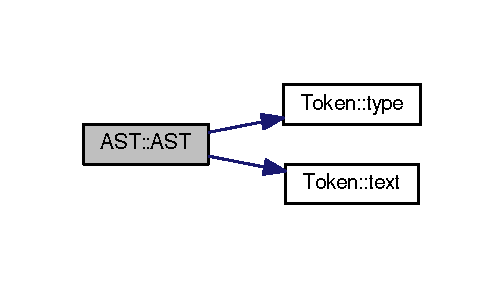
\includegraphics[width=244pt]{class_a_s_t_a039b00473e1617d1c3003b0a22d5f2d9_cgraph}
\end{center}
\end{figure}


\hypertarget{class_a_s_t_a56011c7a97fd6277c72e88c2acd6a96e}{
\index{AST@{AST}!AST@{AST}}
\index{AST@{AST}!AST@{AST}}
\subsubsection[{AST}]{\setlength{\rightskip}{0pt plus 5cm}AST::AST (
\begin{DoxyParamCaption}
\item[{{\bf ASTNodeType}}]{type, }
\item[{const char $\ast$}]{text}
\end{DoxyParamCaption}
)}}
\label{class_a_s_t_a56011c7a97fd6277c72e88c2acd6a96e}


Definition at line 23 of file ast.cpp.

\hypertarget{class_a_s_t_a341ac3dbf80dad18be249944c0b5f222}{
\index{AST@{AST}!AST@{AST}}
\index{AST@{AST}!AST@{AST}}
\subsubsection[{AST}]{\setlength{\rightskip}{0pt plus 5cm}AST::AST (
\begin{DoxyParamCaption}
\item[{{\bf ASTNodeType}}]{type, }
\item[{std::string}]{text}
\end{DoxyParamCaption}
)}}
\label{class_a_s_t_a341ac3dbf80dad18be249944c0b5f222}


Definition at line 30 of file ast.cpp.

\hypertarget{class_a_s_t_a5f463c2fad1523f2dfea906e25e60d91}{
\index{AST@{AST}!AST@{AST}}
\index{AST@{AST}!AST@{AST}}
\subsubsection[{AST}]{\setlength{\rightskip}{0pt plus 5cm}AST::AST (
\begin{DoxyParamCaption}
\item[{{\bf ASTNodeType}}]{type, }
\item[{int}]{child\_\-count, }
\item[{}]{...}
\end{DoxyParamCaption}
)}}
\label{class_a_s_t_a5f463c2fad1523f2dfea906e25e60d91}


Definition at line 37 of file ast.cpp.

\hypertarget{class_a_s_t_aab868b0cf41c496ee5654fb17e61e63c}{
\index{AST@{AST}!AST@{AST}}
\index{AST@{AST}!AST@{AST}}
\subsubsection[{AST}]{\setlength{\rightskip}{0pt plus 5cm}AST::AST (
\begin{DoxyParamCaption}
\item[{{\bf ASTNodeType}}]{type, }
\item[{std::string}]{text, }
\item[{int}]{child\_\-count, }
\item[{}]{...}
\end{DoxyParamCaption}
)}}
\label{class_a_s_t_aab868b0cf41c496ee5654fb17e61e63c}


Definition at line 52 of file ast.cpp.

\hypertarget{class_a_s_t_ad332977af5d4ea0ec793c4843544b6e2}{
\index{AST@{AST}!$\sim$AST@{$\sim$AST}}
\index{$\sim$AST@{$\sim$AST}!AST@{AST}}
\subsubsection[{$\sim$AST}]{\setlength{\rightskip}{0pt plus 5cm}AST::$\sim$AST (
\begin{DoxyParamCaption}
{}
\end{DoxyParamCaption}
)\hspace{0.3cm}{\ttfamily  \mbox{[}virtual\mbox{]}}}}
\label{class_a_s_t_ad332977af5d4ea0ec793c4843544b6e2}


Definition at line 67 of file ast.cpp.



\subsection{Member Function Documentation}
\hypertarget{class_a_s_t_a131ed8cb88639003df1058f768820cc5}{
\index{AST@{AST}!addChild@{addChild}}
\index{addChild@{addChild}!AST@{AST}}
\subsubsection[{addChild}]{\setlength{\rightskip}{0pt plus 5cm}void AST::addChild (
\begin{DoxyParamCaption}
\item[{{\bf AST} $\ast$}]{node}
\end{DoxyParamCaption}
)}}
\label{class_a_s_t_a131ed8cb88639003df1058f768820cc5}


Definition at line 117 of file ast.cpp.



Here is the caller graph for this function:\nopagebreak
\begin{figure}[H]
\begin{center}
\leavevmode
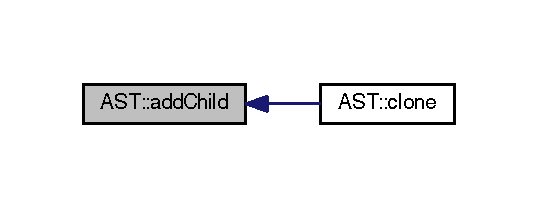
\includegraphics[width=262pt]{class_a_s_t_a131ed8cb88639003df1058f768820cc5_icgraph}
\end{center}
\end{figure}


\hypertarget{class_a_s_t_addfd95ed0ba31ec4fdcf08097fb7fa75}{
\index{AST@{AST}!children@{children}}
\index{children@{children}!AST@{AST}}
\subsubsection[{children}]{\setlength{\rightskip}{0pt plus 5cm}list$<$ {\bf AST} $\ast$ $>$ $\ast$ AST::children (
\begin{DoxyParamCaption}
\item[{void}]{}
\end{DoxyParamCaption}
) const}}
\label{class_a_s_t_addfd95ed0ba31ec4fdcf08097fb7fa75}


Definition at line 102 of file ast.cpp.



Here is the caller graph for this function:\nopagebreak
\begin{figure}[H]
\begin{center}
\leavevmode
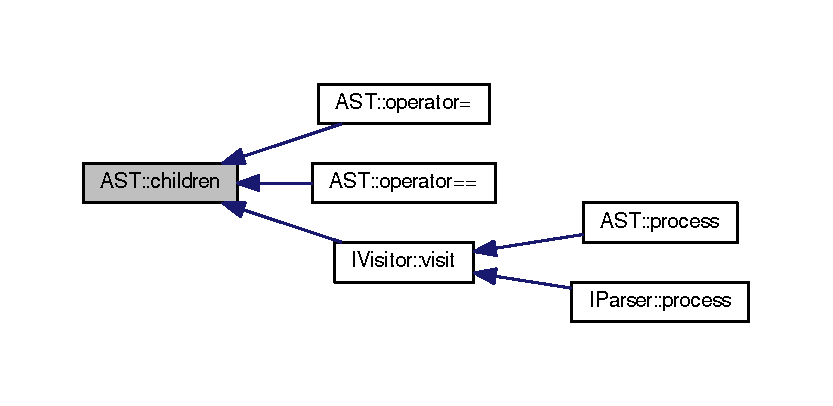
\includegraphics[width=400pt]{class_a_s_t_addfd95ed0ba31ec4fdcf08097fb7fa75_icgraph}
\end{center}
\end{figure}


\hypertarget{class_a_s_t_a787d24b79bf03b6ae15f10d9fad3411b}{
\index{AST@{AST}!clone@{clone}}
\index{clone@{clone}!AST@{AST}}
\subsubsection[{clone}]{\setlength{\rightskip}{0pt plus 5cm}{\bf AST} $\ast$ AST::clone (
\begin{DoxyParamCaption}
\item[{void}]{}
\end{DoxyParamCaption}
) const}}
\label{class_a_s_t_a787d24b79bf03b6ae15f10d9fad3411b}


Definition at line 122 of file ast.cpp.



Here is the call graph for this function:\nopagebreak
\begin{figure}[H]
\begin{center}
\leavevmode
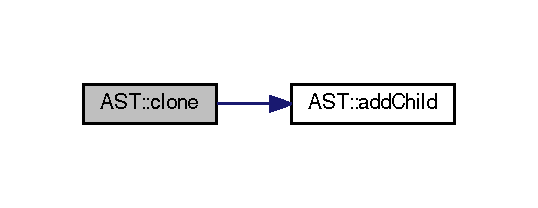
\includegraphics[width=262pt]{class_a_s_t_a787d24b79bf03b6ae15f10d9fad3411b_cgraph}
\end{center}
\end{figure}


\hypertarget{class_a_s_t_a00250cbeed3c73d95d4117b20d8146dd}{
\index{AST@{AST}!operator!=@{operator!=}}
\index{operator!=@{operator!=}!AST@{AST}}
\subsubsection[{operator!=}]{\setlength{\rightskip}{0pt plus 5cm}bool AST::operator!= (
\begin{DoxyParamCaption}
\item[{const {\bf AST} \&}]{other}
\end{DoxyParamCaption}
) const}}
\label{class_a_s_t_a00250cbeed3c73d95d4117b20d8146dd}


Definition at line 168 of file ast.cpp.

\hypertarget{class_a_s_t_aa28dd92452d4f89c16a4de0058905e16}{
\index{AST@{AST}!operator=@{operator=}}
\index{operator=@{operator=}!AST@{AST}}
\subsubsection[{operator=}]{\setlength{\rightskip}{0pt plus 5cm}{\bf AST} \& AST::operator= (
\begin{DoxyParamCaption}
\item[{{\bf AST} \&}]{rhs}
\end{DoxyParamCaption}
)}}
\label{class_a_s_t_aa28dd92452d4f89c16a4de0058905e16}


Definition at line 77 of file ast.cpp.



Here is the call graph for this function:\nopagebreak
\begin{figure}[H]
\begin{center}
\leavevmode
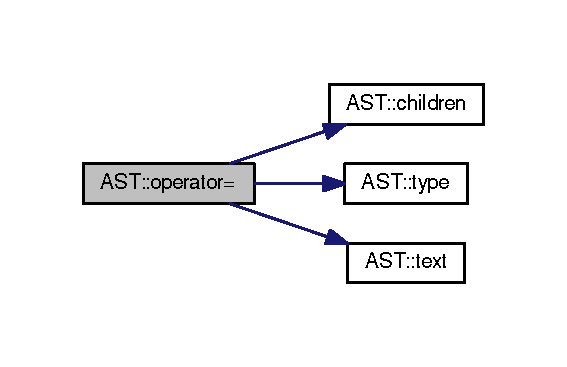
\includegraphics[width=276pt]{class_a_s_t_aa28dd92452d4f89c16a4de0058905e16_cgraph}
\end{center}
\end{figure}


\hypertarget{class_a_s_t_a2329c4b895ed7832713563d00b89e978}{
\index{AST@{AST}!operator==@{operator==}}
\index{operator==@{operator==}!AST@{AST}}
\subsubsection[{operator==}]{\setlength{\rightskip}{0pt plus 5cm}bool AST::operator== (
\begin{DoxyParamCaption}
\item[{const {\bf AST} \&}]{other}
\end{DoxyParamCaption}
) const}}
\label{class_a_s_t_a2329c4b895ed7832713563d00b89e978}


Definition at line 133 of file ast.cpp.



Here is the call graph for this function:\nopagebreak
\begin{figure}[H]
\begin{center}
\leavevmode
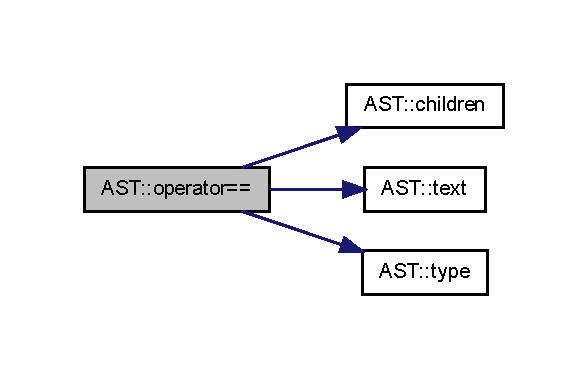
\includegraphics[width=282pt]{class_a_s_t_a2329c4b895ed7832713563d00b89e978_cgraph}
\end{center}
\end{figure}


\hypertarget{class_a_s_t_af8504282645b3e5baebabc486877ea1e}{
\index{AST@{AST}!process@{process}}
\index{process@{process}!AST@{AST}}
\subsubsection[{process}]{\setlength{\rightskip}{0pt plus 5cm}void AST::process (
\begin{DoxyParamCaption}
\item[{{\bf IVisitor} \&}]{visitor}
\end{DoxyParamCaption}
)}}
\label{class_a_s_t_af8504282645b3e5baebabc486877ea1e}


Definition at line 173 of file ast.cpp.



Here is the call graph for this function:\nopagebreak
\begin{figure}[H]
\begin{center}
\leavevmode
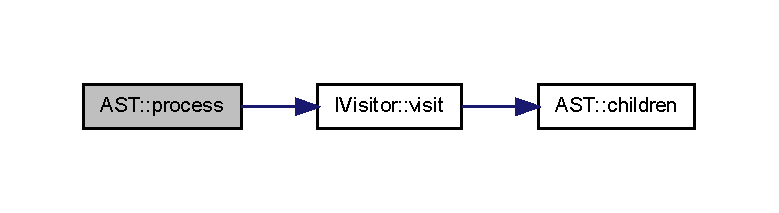
\includegraphics[width=374pt]{class_a_s_t_af8504282645b3e5baebabc486877ea1e_cgraph}
\end{center}
\end{figure}


\hypertarget{class_a_s_t_a5b90708376a408b1e1ff5762975017e9}{
\index{AST@{AST}!text@{text}}
\index{text@{text}!AST@{AST}}
\subsubsection[{text}]{\setlength{\rightskip}{0pt plus 5cm}void AST::text (
\begin{DoxyParamCaption}
\item[{std::string \&}]{txt}
\end{DoxyParamCaption}
)}}
\label{class_a_s_t_a5b90708376a408b1e1ff5762975017e9}


Definition at line 112 of file ast.cpp.

\hypertarget{class_a_s_t_ad975048d27d24ffe87e95b1eed995d5e}{
\index{AST@{AST}!text@{text}}
\index{text@{text}!AST@{AST}}
\subsubsection[{text}]{\setlength{\rightskip}{0pt plus 5cm}string AST::text (
\begin{DoxyParamCaption}
\item[{void}]{}
\end{DoxyParamCaption}
) const}}
\label{class_a_s_t_ad975048d27d24ffe87e95b1eed995d5e}


Definition at line 107 of file ast.cpp.



Here is the caller graph for this function:\nopagebreak
\begin{figure}[H]
\begin{center}
\leavevmode
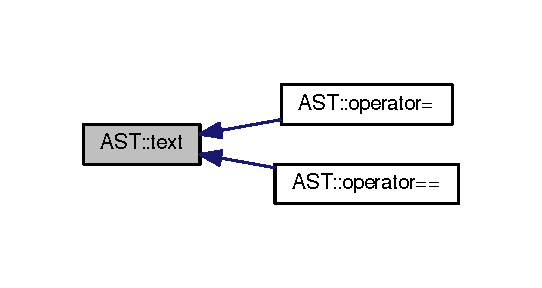
\includegraphics[width=264pt]{class_a_s_t_ad975048d27d24ffe87e95b1eed995d5e_icgraph}
\end{center}
\end{figure}


\hypertarget{class_a_s_t_a3bf7042778ad5c589b65dd1b276f093c}{
\index{AST@{AST}!type@{type}}
\index{type@{type}!AST@{AST}}
\subsubsection[{type}]{\setlength{\rightskip}{0pt plus 5cm}void AST::type (
\begin{DoxyParamCaption}
\item[{{\bf ASTNodeType}}]{typ}
\end{DoxyParamCaption}
)}}
\label{class_a_s_t_a3bf7042778ad5c589b65dd1b276f093c}


Definition at line 97 of file ast.cpp.

\hypertarget{class_a_s_t_ad947af30e5dbb743c41769296dc03c9d}{
\index{AST@{AST}!type@{type}}
\index{type@{type}!AST@{AST}}
\subsubsection[{type}]{\setlength{\rightskip}{0pt plus 5cm}{\bf ASTNodeType} AST::type (
\begin{DoxyParamCaption}
\item[{void}]{}
\end{DoxyParamCaption}
) const}}
\label{class_a_s_t_ad947af30e5dbb743c41769296dc03c9d}


Definition at line 92 of file ast.cpp.



Here is the caller graph for this function:\nopagebreak
\begin{figure}[H]
\begin{center}
\leavevmode
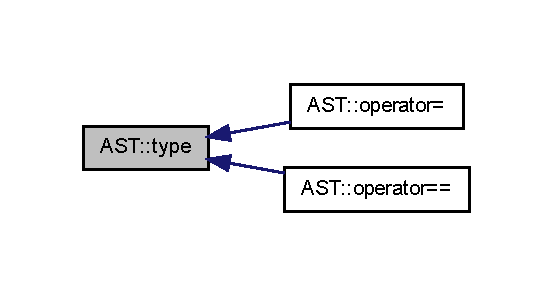
\includegraphics[width=266pt]{class_a_s_t_ad947af30e5dbb743c41769296dc03c9d_icgraph}
\end{center}
\end{figure}




\subsection{Member Data Documentation}
\hypertarget{class_a_s_t_acb9265830632be3a68812c66c08c8752}{
\index{AST@{AST}!node\_\-children@{node\_\-children}}
\index{node\_\-children@{node\_\-children}!AST@{AST}}
\subsubsection[{node\_\-children}]{\setlength{\rightskip}{0pt plus 5cm}std::list$<${\bf AST}$\ast$$>$$\ast$ {\bf AST::node\_\-children}\hspace{0.3cm}{\ttfamily  \mbox{[}protected\mbox{]}}}}
\label{class_a_s_t_acb9265830632be3a68812c66c08c8752}


Definition at line 19 of file ast.h.

\hypertarget{class_a_s_t_a1638e0900cea081df5bb23d76432a2c3}{
\index{AST@{AST}!node\_\-text@{node\_\-text}}
\index{node\_\-text@{node\_\-text}!AST@{AST}}
\subsubsection[{node\_\-text}]{\setlength{\rightskip}{0pt plus 5cm}std::string {\bf AST::node\_\-text}\hspace{0.3cm}{\ttfamily  \mbox{[}protected\mbox{]}}}}
\label{class_a_s_t_a1638e0900cea081df5bb23d76432a2c3}


Definition at line 18 of file ast.h.

\hypertarget{class_a_s_t_aa650b2056cd9f76cc9b8833ca5faf312}{
\index{AST@{AST}!node\_\-type@{node\_\-type}}
\index{node\_\-type@{node\_\-type}!AST@{AST}}
\subsubsection[{node\_\-type}]{\setlength{\rightskip}{0pt plus 5cm}{\bf ASTNodeType} {\bf AST::node\_\-type}\hspace{0.3cm}{\ttfamily  \mbox{[}protected\mbox{]}}}}
\label{class_a_s_t_aa650b2056cd9f76cc9b8833ca5faf312}


Definition at line 17 of file ast.h.



The documentation for this class was generated from the following files:\begin{DoxyCompactItemize}
\item 
source/parser/ast/\hyperlink{ast_8h}{ast.h}\item 
source/parser/ast/\hyperlink{ast_8cpp}{ast.cpp}\end{DoxyCompactItemize}

\hypertarget{class_a_s_t_printer}{\section{A\-S\-T\-Printer Class Reference}
\label{class_a_s_t_printer}\index{A\-S\-T\-Printer@{A\-S\-T\-Printer}}
}


{\ttfamily \#include $<$astprinter.\-h$>$}



Inheritance diagram for A\-S\-T\-Printer\-:
\nopagebreak
\begin{figure}[H]
\begin{center}
\leavevmode
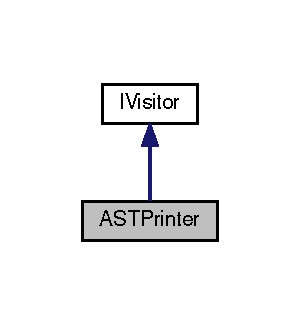
\includegraphics[width=144pt]{class_a_s_t_printer__inherit__graph}
\end{center}
\end{figure}


Collaboration diagram for A\-S\-T\-Printer\-:
\nopagebreak
\begin{figure}[H]
\begin{center}
\leavevmode
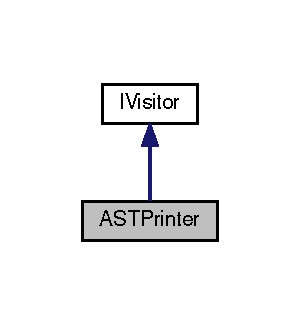
\includegraphics[width=144pt]{class_a_s_t_printer__coll__graph}
\end{center}
\end{figure}
\subsection*{Additional Inherited Members}


\subsection{Detailed Description}


Definition at line 8 of file astprinter.\-h.



The documentation for this class was generated from the following files\-:\begin{DoxyCompactItemize}
\item 
source/visitor/astprinter/\hyperlink{astprinter_8h}{astprinter.\-h}\item 
source/visitor/astprinter/\hyperlink{astprinter_8cpp}{astprinter.\-cpp}\end{DoxyCompactItemize}

\hypertarget{class_b_t_parser}{
\section{BTParser Class Reference}
\label{class_b_t_parser}\index{BTParser@{BTParser}}
}


{\ttfamily \#include $<$btparser.h$>$}



Inheritance diagram for BTParser:
\nopagebreak
\begin{figure}[H]
\begin{center}
\leavevmode
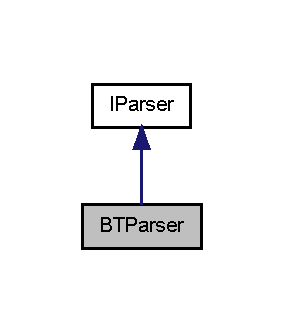
\includegraphics[width=192pt]{class_b_t_parser__inherit__graph}
\end{center}
\end{figure}


Collaboration diagram for BTParser:
\nopagebreak
\begin{figure}[H]
\begin{center}
\leavevmode
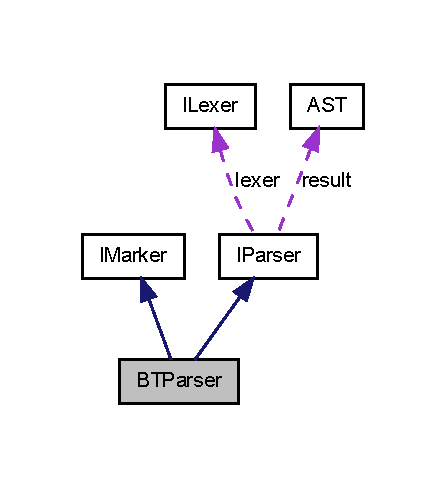
\includegraphics[width=214pt]{class_b_t_parser__coll__graph}
\end{center}
\end{figure}
\subsection*{Public Member Functions}
\begin{DoxyCompactItemize}
\item 
\hyperlink{class_b_t_parser_ad9495eabeaf69d91c5f26131cabd3ec4}{BTParser} ()
\item 
virtual \hyperlink{class_b_t_parser_a5965c4cf0baf950be976a0a2932eec2c}{$\sim$BTParser} ()
\item 
void \hyperlink{class_b_t_parser_a9d72bba86b16427b0b03e91113b0f027}{consume} (void)
\item 
void \hyperlink{class_b_t_parser_a762e16322aec6e50af51c2b6377d86fe}{sync} (unsigned int i)
\item 
void \hyperlink{class_b_t_parser_a366b4477388d2cd7fd655b36342f882c}{fill} (unsigned int n)
\item 
void \hyperlink{class_b_t_parser_ad8fb9348dd9bc2e65a08033dd2539a03}{match} (\hyperlink{token_8h_abf05bcc4c1b09928131e6afd3b768a77}{TokenType\_\-T} type)
\item 
\hyperlink{class_token}{Token} \& \hyperlink{class_b_t_parser_a2674f280bd3000751a100b45ac3899e2}{lookaheadToken} (unsigned int i)
\item 
\hyperlink{token_8h_abf05bcc4c1b09928131e6afd3b768a77}{TokenType\_\-T} \hyperlink{class_b_t_parser_a01abded048ed1573e03867f7f2316583}{lookaheadType} (unsigned int i)
\end{DoxyCompactItemize}
\subsection*{Protected Attributes}
\begin{DoxyCompactItemize}
\item 
std::vector$<$ \hyperlink{class_token}{Token} $>$ \hyperlink{class_b_t_parser_a796693745ebe354914eeacddba20f109}{lookahead}
\end{DoxyCompactItemize}


\subsection{Detailed Description}


Definition at line 9 of file btparser.h.



\subsection{Constructor \& Destructor Documentation}
\hypertarget{class_b_t_parser_ad9495eabeaf69d91c5f26131cabd3ec4}{
\index{BTParser@{BTParser}!BTParser@{BTParser}}
\index{BTParser@{BTParser}!BTParser@{BTParser}}
\subsubsection[{BTParser}]{\setlength{\rightskip}{0pt plus 5cm}BTParser::BTParser (
\begin{DoxyParamCaption}
{}
\end{DoxyParamCaption}
)}}
\label{class_b_t_parser_ad9495eabeaf69d91c5f26131cabd3ec4}


Definition at line 6 of file btparser.cpp.

\hypertarget{class_b_t_parser_a5965c4cf0baf950be976a0a2932eec2c}{
\index{BTParser@{BTParser}!$\sim$BTParser@{$\sim$BTParser}}
\index{$\sim$BTParser@{$\sim$BTParser}!BTParser@{BTParser}}
\subsubsection[{$\sim$BTParser}]{\setlength{\rightskip}{0pt plus 5cm}BTParser::$\sim$BTParser (
\begin{DoxyParamCaption}
{}
\end{DoxyParamCaption}
)\hspace{0.3cm}{\ttfamily  \mbox{[}virtual\mbox{]}}}}
\label{class_b_t_parser_a5965c4cf0baf950be976a0a2932eec2c}


Definition at line 10 of file btparser.cpp.



\subsection{Member Function Documentation}
\hypertarget{class_b_t_parser_a9d72bba86b16427b0b03e91113b0f027}{
\index{BTParser@{BTParser}!consume@{consume}}
\index{consume@{consume}!BTParser@{BTParser}}
\subsubsection[{consume}]{\setlength{\rightskip}{0pt plus 5cm}void BTParser::consume (
\begin{DoxyParamCaption}
\item[{void}]{}
\end{DoxyParamCaption}
)}}
\label{class_b_t_parser_a9d72bba86b16427b0b03e91113b0f027}


Definition at line 14 of file btparser.cpp.

\hypertarget{class_b_t_parser_a366b4477388d2cd7fd655b36342f882c}{
\index{BTParser@{BTParser}!fill@{fill}}
\index{fill@{fill}!BTParser@{BTParser}}
\subsubsection[{fill}]{\setlength{\rightskip}{0pt plus 5cm}void BTParser::fill (
\begin{DoxyParamCaption}
\item[{unsigned int}]{n}
\end{DoxyParamCaption}
)}}
\label{class_b_t_parser_a366b4477388d2cd7fd655b36342f882c}


Definition at line 40 of file btparser.cpp.

\hypertarget{class_b_t_parser_a2674f280bd3000751a100b45ac3899e2}{
\index{BTParser@{BTParser}!lookaheadToken@{lookaheadToken}}
\index{lookaheadToken@{lookaheadToken}!BTParser@{BTParser}}
\subsubsection[{lookaheadToken}]{\setlength{\rightskip}{0pt plus 5cm}{\bf Token} \& BTParser::lookaheadToken (
\begin{DoxyParamCaption}
\item[{unsigned int}]{i}
\end{DoxyParamCaption}
)}}
\label{class_b_t_parser_a2674f280bd3000751a100b45ac3899e2}


Definition at line 63 of file btparser.cpp.

\hypertarget{class_b_t_parser_a01abded048ed1573e03867f7f2316583}{
\index{BTParser@{BTParser}!lookaheadType@{lookaheadType}}
\index{lookaheadType@{lookaheadType}!BTParser@{BTParser}}
\subsubsection[{lookaheadType}]{\setlength{\rightskip}{0pt plus 5cm}{\bf TokenType\_\-T} BTParser::lookaheadType (
\begin{DoxyParamCaption}
\item[{unsigned int}]{i}
\end{DoxyParamCaption}
)}}
\label{class_b_t_parser_a01abded048ed1573e03867f7f2316583}


Definition at line 69 of file btparser.cpp.

\hypertarget{class_b_t_parser_ad8fb9348dd9bc2e65a08033dd2539a03}{
\index{BTParser@{BTParser}!match@{match}}
\index{match@{match}!BTParser@{BTParser}}
\subsubsection[{match}]{\setlength{\rightskip}{0pt plus 5cm}void BTParser::match (
\begin{DoxyParamCaption}
\item[{{\bf TokenType\_\-T}}]{type}
\end{DoxyParamCaption}
)}}
\label{class_b_t_parser_ad8fb9348dd9bc2e65a08033dd2539a03}


Definition at line 49 of file btparser.cpp.

\hypertarget{class_b_t_parser_a762e16322aec6e50af51c2b6377d86fe}{
\index{BTParser@{BTParser}!sync@{sync}}
\index{sync@{sync}!BTParser@{BTParser}}
\subsubsection[{sync}]{\setlength{\rightskip}{0pt plus 5cm}void BTParser::sync (
\begin{DoxyParamCaption}
\item[{unsigned int}]{i}
\end{DoxyParamCaption}
)}}
\label{class_b_t_parser_a762e16322aec6e50af51c2b6377d86fe}


Definition at line 25 of file btparser.cpp.



\subsection{Member Data Documentation}
\hypertarget{class_b_t_parser_a796693745ebe354914eeacddba20f109}{
\index{BTParser@{BTParser}!lookahead@{lookahead}}
\index{lookahead@{lookahead}!BTParser@{BTParser}}
\subsubsection[{lookahead}]{\setlength{\rightskip}{0pt plus 5cm}std::vector$<${\bf Token}$>$ {\bf BTParser::lookahead}\hspace{0.3cm}{\ttfamily  \mbox{[}protected\mbox{]}}}}
\label{class_b_t_parser_a796693745ebe354914eeacddba20f109}


Definition at line 14 of file btparser.h.



The documentation for this class was generated from the following files:\begin{DoxyCompactItemize}
\item 
source/parser/btparser/\hyperlink{btparser_8h}{btparser.h}\item 
source/parser/btparser/\hyperlink{btparser_8cpp}{btparser.cpp}\end{DoxyCompactItemize}

\hypertarget{class_exception}{\section{Exception Class Reference}
\label{class_exception}\index{Exception@{Exception}}
}


{\ttfamily \#include $<$exception.\-h$>$}

\subsection*{Public Member Functions}
\begin{DoxyCompactItemize}
\item 
\hyperlink{class_exception_a1b78336bb26edf8e784783cc150c5801}{Exception} ()  throw ()
\item 
\hyperlink{class_exception_abfa91380075acb0b040b401ace9885d8}{Exception} (const \hyperlink{class_token}{Token} \&tok)  throw ()
\item 
\hyperlink{class_exception_aa049354d27370ca0176a16c5ed7394e9}{Exception} (int line, int column)  throw ()
\item 
virtual \hyperlink{class_exception_ad1ba411de295ef2eeb02ba26284a829a}{$\sim$\-Exception} ()  throw ()
\item 
virtual const char $\ast$ \hyperlink{class_exception_a380f0477d9ef319911e7a8167bd47f1f}{what} () const   throw ()
\item 
void \hyperlink{class_exception_a2514fc52bf060e2d242f5e6f1b87e8bf}{message} (const std\-::string \&msg)  throw ()
\item 
const std\-::string \& \hyperlink{class_exception_a8f4eb20583b892ce7b0fb55554a94156}{message} (void) const   throw ()
\end{DoxyCompactItemize}
\subsection*{Protected Attributes}
\begin{DoxyCompactItemize}
\item 
int \hyperlink{class_exception_ab30bf54ebcf9ead45300ce422fb4b6b8}{ex\-\_\-line}
\item 
int \hyperlink{class_exception_a5a08b0f7c24a639573c36ace567348c4}{ex\-\_\-column}
\item 
std\-::string \hyperlink{class_exception_ac106ae3b8d10ae97ee0b71a270fbda27}{ex\-\_\-msg}
\end{DoxyCompactItemize}
\subsection*{Friends}
\begin{DoxyCompactItemize}
\item 
\hyperlink{class_exception}{Exception} \& \hyperlink{class_exception_a14ad8d29bc8d9f4eb8d2a0b0e5b1047f}{operator$<$$<$} (\hyperlink{class_exception}{Exception} \&ex, const std\-::string \&rhs)
\item 
\hyperlink{class_exception}{Exception} \& \hyperlink{class_exception_a96bb231c8f8c68239c83b6fa691e02b4}{operator$<$$<$} (\hyperlink{class_exception}{Exception} \&ex, unsigned int rhs)
\end{DoxyCompactItemize}


\subsection{Detailed Description}


Definition at line 8 of file exception.\-h.



\subsection{Constructor \& Destructor Documentation}
\hypertarget{class_exception_a1b78336bb26edf8e784783cc150c5801}{\index{Exception@{Exception}!Exception@{Exception}}
\index{Exception@{Exception}!Exception@{Exception}}
\subsubsection[{Exception}]{\setlength{\rightskip}{0pt plus 5cm}Exception\-::\-Exception (
\begin{DoxyParamCaption}
{}
\end{DoxyParamCaption}
)  throw ()}}\label{class_exception_a1b78336bb26edf8e784783cc150c5801}


Definition at line 4 of file exception.\-cpp.

\hypertarget{class_exception_abfa91380075acb0b040b401ace9885d8}{\index{Exception@{Exception}!Exception@{Exception}}
\index{Exception@{Exception}!Exception@{Exception}}
\subsubsection[{Exception}]{\setlength{\rightskip}{0pt plus 5cm}Exception\-::\-Exception (
\begin{DoxyParamCaption}
\item[{const {\bf Token} \&}]{tok}
\end{DoxyParamCaption}
)  throw ()}}\label{class_exception_abfa91380075acb0b040b401ace9885d8}


Definition at line 8 of file exception.\-cpp.

\hypertarget{class_exception_aa049354d27370ca0176a16c5ed7394e9}{\index{Exception@{Exception}!Exception@{Exception}}
\index{Exception@{Exception}!Exception@{Exception}}
\subsubsection[{Exception}]{\setlength{\rightskip}{0pt plus 5cm}Exception\-::\-Exception (
\begin{DoxyParamCaption}
\item[{int}]{line, }
\item[{int}]{column}
\end{DoxyParamCaption}
)  throw ()}}\label{class_exception_aa049354d27370ca0176a16c5ed7394e9}


Definition at line 16 of file exception.\-cpp.

\hypertarget{class_exception_ad1ba411de295ef2eeb02ba26284a829a}{\index{Exception@{Exception}!$\sim$\-Exception@{$\sim$\-Exception}}
\index{$\sim$\-Exception@{$\sim$\-Exception}!Exception@{Exception}}
\subsubsection[{$\sim$\-Exception}]{\setlength{\rightskip}{0pt plus 5cm}virtual Exception\-::$\sim$\-Exception (
\begin{DoxyParamCaption}
{}
\end{DoxyParamCaption}
)  throw ()\hspace{0.3cm}{\ttfamily [inline]}, {\ttfamily [virtual]}}}\label{class_exception_ad1ba411de295ef2eeb02ba26284a829a}


Definition at line 18 of file exception.\-h.



\subsection{Member Function Documentation}
\hypertarget{class_exception_a2514fc52bf060e2d242f5e6f1b87e8bf}{\index{Exception@{Exception}!message@{message}}
\index{message@{message}!Exception@{Exception}}
\subsubsection[{message}]{\setlength{\rightskip}{0pt plus 5cm}void Exception\-::message (
\begin{DoxyParamCaption}
\item[{const std\-::string \&}]{msg}
\end{DoxyParamCaption}
)  throw ()}}\label{class_exception_a2514fc52bf060e2d242f5e6f1b87e8bf}


Definition at line 29 of file exception.\-cpp.

\hypertarget{class_exception_a8f4eb20583b892ce7b0fb55554a94156}{\index{Exception@{Exception}!message@{message}}
\index{message@{message}!Exception@{Exception}}
\subsubsection[{message}]{\setlength{\rightskip}{0pt plus 5cm}const std\-::string \& Exception\-::message (
\begin{DoxyParamCaption}
\item[{void}]{}
\end{DoxyParamCaption}
) const  throw ()}}\label{class_exception_a8f4eb20583b892ce7b0fb55554a94156}


Definition at line 34 of file exception.\-cpp.

\hypertarget{class_exception_a380f0477d9ef319911e7a8167bd47f1f}{\index{Exception@{Exception}!what@{what}}
\index{what@{what}!Exception@{Exception}}
\subsubsection[{what}]{\setlength{\rightskip}{0pt plus 5cm}const char $\ast$ Exception\-::what (
\begin{DoxyParamCaption}
{}
\end{DoxyParamCaption}
) const  throw ()\hspace{0.3cm}{\ttfamily [virtual]}}}\label{class_exception_a380f0477d9ef319911e7a8167bd47f1f}


Definition at line 24 of file exception.\-cpp.



\subsection{Friends And Related Function Documentation}
\hypertarget{class_exception_a14ad8d29bc8d9f4eb8d2a0b0e5b1047f}{\index{Exception@{Exception}!operator$<$$<$@{operator$<$$<$}}
\index{operator$<$$<$@{operator$<$$<$}!Exception@{Exception}}
\subsubsection[{operator$<$$<$}]{\setlength{\rightskip}{0pt plus 5cm}{\bf Exception}\& operator$<$$<$ (
\begin{DoxyParamCaption}
\item[{{\bf Exception} \&}]{ex, }
\item[{const std\-::string \&}]{rhs}
\end{DoxyParamCaption}
)\hspace{0.3cm}{\ttfamily [friend]}}}\label{class_exception_a14ad8d29bc8d9f4eb8d2a0b0e5b1047f}


Definition at line 39 of file exception.\-cpp.

\hypertarget{class_exception_a96bb231c8f8c68239c83b6fa691e02b4}{\index{Exception@{Exception}!operator$<$$<$@{operator$<$$<$}}
\index{operator$<$$<$@{operator$<$$<$}!Exception@{Exception}}
\subsubsection[{operator$<$$<$}]{\setlength{\rightskip}{0pt plus 5cm}{\bf Exception}\& operator$<$$<$ (
\begin{DoxyParamCaption}
\item[{{\bf Exception} \&}]{ex, }
\item[{unsigned int}]{rhs}
\end{DoxyParamCaption}
)\hspace{0.3cm}{\ttfamily [friend]}}}\label{class_exception_a96bb231c8f8c68239c83b6fa691e02b4}


Definition at line 45 of file exception.\-cpp.



\subsection{Member Data Documentation}
\hypertarget{class_exception_a5a08b0f7c24a639573c36ace567348c4}{\index{Exception@{Exception}!ex\-\_\-column@{ex\-\_\-column}}
\index{ex\-\_\-column@{ex\-\_\-column}!Exception@{Exception}}
\subsubsection[{ex\-\_\-column}]{\setlength{\rightskip}{0pt plus 5cm}int Exception\-::ex\-\_\-column\hspace{0.3cm}{\ttfamily [protected]}}}\label{class_exception_a5a08b0f7c24a639573c36ace567348c4}


Definition at line 12 of file exception.\-h.

\hypertarget{class_exception_ab30bf54ebcf9ead45300ce422fb4b6b8}{\index{Exception@{Exception}!ex\-\_\-line@{ex\-\_\-line}}
\index{ex\-\_\-line@{ex\-\_\-line}!Exception@{Exception}}
\subsubsection[{ex\-\_\-line}]{\setlength{\rightskip}{0pt plus 5cm}int Exception\-::ex\-\_\-line\hspace{0.3cm}{\ttfamily [protected]}}}\label{class_exception_ab30bf54ebcf9ead45300ce422fb4b6b8}


Definition at line 11 of file exception.\-h.

\hypertarget{class_exception_ac106ae3b8d10ae97ee0b71a270fbda27}{\index{Exception@{Exception}!ex\-\_\-msg@{ex\-\_\-msg}}
\index{ex\-\_\-msg@{ex\-\_\-msg}!Exception@{Exception}}
\subsubsection[{ex\-\_\-msg}]{\setlength{\rightskip}{0pt plus 5cm}std\-::string Exception\-::ex\-\_\-msg\hspace{0.3cm}{\ttfamily [protected]}}}\label{class_exception_ac106ae3b8d10ae97ee0b71a270fbda27}


Definition at line 13 of file exception.\-h.



The documentation for this class was generated from the following files\-:\begin{DoxyCompactItemize}
\item 
source/exception/\hyperlink{exception_8h}{exception.\-h}\item 
source/exception/\hyperlink{exception_8cpp}{exception.\-cpp}\end{DoxyCompactItemize}

\hypertarget{class_i_lexer}{
\section{ILexer Class Reference}
\label{class_i_lexer}\index{ILexer@{ILexer}}
}


{\ttfamily \#include $<$ilexer.h$>$}



Inheritance diagram for ILexer:\nopagebreak
\begin{figure}[H]
\begin{center}
\leavevmode
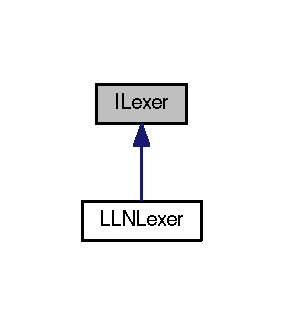
\includegraphics[width=138pt]{class_i_lexer__inherit__graph}
\end{center}
\end{figure}
\subsection*{Public Member Functions}
\begin{DoxyCompactItemize}
\item 
\hyperlink{class_i_lexer_a204cc87b6147aa741d8fde4825843761}{ILexer} (std::istream \&in)
\item 
virtual \hyperlink{class_i_lexer_a1018ca7c4ec102150fe2f6acfe38929d}{$\sim$ILexer} ()
\item 
virtual void \hyperlink{class_i_lexer_ae1009b9b2a1e023e1a7d2fd75806607f}{consume} (void)=0
\item 
virtual void \hyperlink{class_i_lexer_a556fdc7b13486f03cb7c3d7d4612666c}{match} (char x)=0
\item 
virtual bool \hyperlink{class_i_lexer_a0366072c45083ee20123f2552a95b6e0}{eof} (void)
\item 
virtual \hyperlink{class_token}{Token} \hyperlink{class_i_lexer_a6f5098fda43f68b01d2e7a2a7158c50d}{next} (void)=0
\end{DoxyCompactItemize}
\subsection*{Protected Attributes}
\begin{DoxyCompactItemize}
\item 
int \hyperlink{class_i_lexer_a5d766f4f4dcc976553ab17a5753ef8ff}{line}
\item 
int \hyperlink{class_i_lexer_a05ce2bfa3595f992618d2a328b66bdfb}{column}
\item 
std::istream \& \hyperlink{class_i_lexer_a02d418cc6fdcbfbf6cad7bf914cce77f}{in\_\-stream}
\end{DoxyCompactItemize}


\subsection{Detailed Description}


Definition at line 9 of file ilexer.h.



\subsection{Constructor \& Destructor Documentation}
\hypertarget{class_i_lexer_a204cc87b6147aa741d8fde4825843761}{
\index{ILexer@{ILexer}!ILexer@{ILexer}}
\index{ILexer@{ILexer}!ILexer@{ILexer}}
\subsubsection[{ILexer}]{\setlength{\rightskip}{0pt plus 5cm}ILexer::ILexer (
\begin{DoxyParamCaption}
\item[{std::istream \&}]{in}
\end{DoxyParamCaption}
)}}
\label{class_i_lexer_a204cc87b6147aa741d8fde4825843761}


Definition at line 6 of file ilexer.cpp.

\hypertarget{class_i_lexer_a1018ca7c4ec102150fe2f6acfe38929d}{
\index{ILexer@{ILexer}!$\sim$ILexer@{$\sim$ILexer}}
\index{$\sim$ILexer@{$\sim$ILexer}!ILexer@{ILexer}}
\subsubsection[{$\sim$ILexer}]{\setlength{\rightskip}{0pt plus 5cm}ILexer::$\sim$ILexer (
\begin{DoxyParamCaption}
{}
\end{DoxyParamCaption}
)\hspace{0.3cm}{\ttfamily  \mbox{[}virtual\mbox{]}}}}
\label{class_i_lexer_a1018ca7c4ec102150fe2f6acfe38929d}


Definition at line 10 of file ilexer.cpp.



\subsection{Member Function Documentation}
\hypertarget{class_i_lexer_ae1009b9b2a1e023e1a7d2fd75806607f}{
\index{ILexer@{ILexer}!consume@{consume}}
\index{consume@{consume}!ILexer@{ILexer}}
\subsubsection[{consume}]{\setlength{\rightskip}{0pt plus 5cm}virtual void ILexer::consume (
\begin{DoxyParamCaption}
\item[{void}]{}
\end{DoxyParamCaption}
)\hspace{0.3cm}{\ttfamily  \mbox{[}pure virtual\mbox{]}}}}
\label{class_i_lexer_ae1009b9b2a1e023e1a7d2fd75806607f}


Implemented in \hyperlink{class_l_l_n_lexer_ada670d39fa588ed793c71fe286ffe01d}{LLNLexer}.

\hypertarget{class_i_lexer_a0366072c45083ee20123f2552a95b6e0}{
\index{ILexer@{ILexer}!eof@{eof}}
\index{eof@{eof}!ILexer@{ILexer}}
\subsubsection[{eof}]{\setlength{\rightskip}{0pt plus 5cm}bool ILexer::eof (
\begin{DoxyParamCaption}
\item[{void}]{}
\end{DoxyParamCaption}
)\hspace{0.3cm}{\ttfamily  \mbox{[}virtual\mbox{]}}}}
\label{class_i_lexer_a0366072c45083ee20123f2552a95b6e0}


Definition at line 14 of file ilexer.cpp.

\hypertarget{class_i_lexer_a556fdc7b13486f03cb7c3d7d4612666c}{
\index{ILexer@{ILexer}!match@{match}}
\index{match@{match}!ILexer@{ILexer}}
\subsubsection[{match}]{\setlength{\rightskip}{0pt plus 5cm}virtual void ILexer::match (
\begin{DoxyParamCaption}
\item[{char}]{x}
\end{DoxyParamCaption}
)\hspace{0.3cm}{\ttfamily  \mbox{[}pure virtual\mbox{]}}}}
\label{class_i_lexer_a556fdc7b13486f03cb7c3d7d4612666c}


Implemented in \hyperlink{class_l_l_n_lexer_a4c250c0e032a7cc3e0ffbdcf8c3b18b7}{LLNLexer}.

\hypertarget{class_i_lexer_a6f5098fda43f68b01d2e7a2a7158c50d}{
\index{ILexer@{ILexer}!next@{next}}
\index{next@{next}!ILexer@{ILexer}}
\subsubsection[{next}]{\setlength{\rightskip}{0pt plus 5cm}virtual {\bf Token} ILexer::next (
\begin{DoxyParamCaption}
\item[{void}]{}
\end{DoxyParamCaption}
)\hspace{0.3cm}{\ttfamily  \mbox{[}pure virtual\mbox{]}}}}
\label{class_i_lexer_a6f5098fda43f68b01d2e7a2a7158c50d}


Implemented in \hyperlink{class_l_l_n_lexer_a3832522afb32a85b3171f552ff9dd676}{LLNLexer}.



Here is the caller graph for this function:
\nopagebreak
\begin{figure}[H]
\begin{center}
\leavevmode
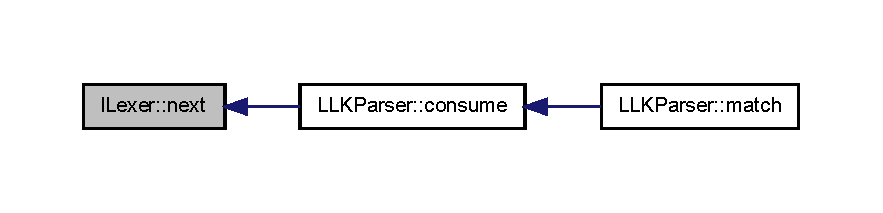
\includegraphics[width=400pt]{class_i_lexer_a6f5098fda43f68b01d2e7a2a7158c50d_icgraph}
\end{center}
\end{figure}




\subsection{Member Data Documentation}
\hypertarget{class_i_lexer_a05ce2bfa3595f992618d2a328b66bdfb}{
\index{ILexer@{ILexer}!column@{column}}
\index{column@{column}!ILexer@{ILexer}}
\subsubsection[{column}]{\setlength{\rightskip}{0pt plus 5cm}int {\bf ILexer::column}\hspace{0.3cm}{\ttfamily  \mbox{[}protected\mbox{]}}}}
\label{class_i_lexer_a05ce2bfa3595f992618d2a328b66bdfb}


Definition at line 13 of file ilexer.h.

\hypertarget{class_i_lexer_a02d418cc6fdcbfbf6cad7bf914cce77f}{
\index{ILexer@{ILexer}!in\_\-stream@{in\_\-stream}}
\index{in\_\-stream@{in\_\-stream}!ILexer@{ILexer}}
\subsubsection[{in\_\-stream}]{\setlength{\rightskip}{0pt plus 5cm}std::istream\& {\bf ILexer::in\_\-stream}\hspace{0.3cm}{\ttfamily  \mbox{[}protected\mbox{]}}}}
\label{class_i_lexer_a02d418cc6fdcbfbf6cad7bf914cce77f}


Definition at line 14 of file ilexer.h.

\hypertarget{class_i_lexer_a5d766f4f4dcc976553ab17a5753ef8ff}{
\index{ILexer@{ILexer}!line@{line}}
\index{line@{line}!ILexer@{ILexer}}
\subsubsection[{line}]{\setlength{\rightskip}{0pt plus 5cm}int {\bf ILexer::line}\hspace{0.3cm}{\ttfamily  \mbox{[}protected\mbox{]}}}}
\label{class_i_lexer_a5d766f4f4dcc976553ab17a5753ef8ff}


Definition at line 12 of file ilexer.h.



The documentation for this class was generated from the following files:\begin{DoxyCompactItemize}
\item 
source/lexer/\hyperlink{ilexer_8h}{ilexer.h}\item 
source/lexer/\hyperlink{ilexer_8cpp}{ilexer.cpp}\end{DoxyCompactItemize}

\hypertarget{class_i_marker}{
\section{IMarker Class Reference}
\label{class_i_marker}\index{IMarker@{IMarker}}
}


{\ttfamily \#include $<$imarker.h$>$}



Inheritance diagram for IMarker:\nopagebreak
\begin{figure}[H]
\begin{center}
\leavevmode
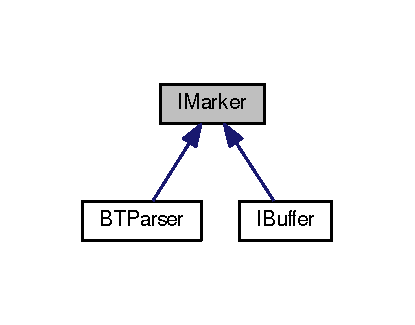
\includegraphics[width=198pt]{class_i_marker__inherit__graph}
\end{center}
\end{figure}
\subsection*{Public Member Functions}
\begin{DoxyCompactItemize}
\item 
\hyperlink{class_i_marker_afbe7a5bbe8cb8f1b86e7ebf7d62782d4}{IMarker} ()
\item 
virtual \hyperlink{class_i_marker_afefb80c6283b5f2327faa16ab131c875}{$\sim$IMarker} ()
\item 
void \hyperlink{class_i_marker_a68c539e79c3052ba7addf090dfd05985}{advance} (void)
\item 
unsigned int \hyperlink{class_i_marker_a0e9628e8c66b493ff331abab55c744da}{location} (void)
\item 
void \hyperlink{class_i_marker_ac2d7a0e8bbfb213378f7a19b50ec9686}{location} (unsigned int index)
\item 
unsigned int \hyperlink{class_i_marker_a92024922612faa5bb0106609f151c050}{mark} (void)
\item 
void \hyperlink{class_i_marker_afce4bb0bef01b4579db97e1ca5e64001}{release} (void)
\item 
void \hyperlink{class_i_marker_a58086bbf091c5b49c15464a070fec171}{seek} (unsigned int index)
\item 
bool \hyperlink{class_i_marker_ae6fda228fa071a9720e7d2309d47ac6e}{isMarked} (void)
\end{DoxyCompactItemize}
\subsection*{Protected Attributes}
\begin{DoxyCompactItemize}
\item 
unsigned int \hyperlink{class_i_marker_adedaefcf6a1b1eac3d728a9d318dc618}{cur\_\-location}
\item 
std::vector$<$ unsigned int $>$ \hyperlink{class_i_marker_a1c1b6ba790e3adf5fa8d9b24c06b10d7}{markers}
\end{DoxyCompactItemize}


\subsection{Detailed Description}


Definition at line 6 of file imarker.h.



\subsection{Constructor \& Destructor Documentation}
\hypertarget{class_i_marker_afbe7a5bbe8cb8f1b86e7ebf7d62782d4}{
\index{IMarker@{IMarker}!IMarker@{IMarker}}
\index{IMarker@{IMarker}!IMarker@{IMarker}}
\subsubsection[{IMarker}]{\setlength{\rightskip}{0pt plus 5cm}IMarker::IMarker (
\begin{DoxyParamCaption}
{}
\end{DoxyParamCaption}
)}}
\label{class_i_marker_afbe7a5bbe8cb8f1b86e7ebf7d62782d4}


Definition at line 3 of file imarker.cpp.

\hypertarget{class_i_marker_afefb80c6283b5f2327faa16ab131c875}{
\index{IMarker@{IMarker}!$\sim$IMarker@{$\sim$IMarker}}
\index{$\sim$IMarker@{$\sim$IMarker}!IMarker@{IMarker}}
\subsubsection[{$\sim$IMarker}]{\setlength{\rightskip}{0pt plus 5cm}IMarker::$\sim$IMarker (
\begin{DoxyParamCaption}
{}
\end{DoxyParamCaption}
)\hspace{0.3cm}{\ttfamily  \mbox{[}virtual\mbox{]}}}}
\label{class_i_marker_afefb80c6283b5f2327faa16ab131c875}


Definition at line 7 of file imarker.cpp.



\subsection{Member Function Documentation}
\hypertarget{class_i_marker_a68c539e79c3052ba7addf090dfd05985}{
\index{IMarker@{IMarker}!advance@{advance}}
\index{advance@{advance}!IMarker@{IMarker}}
\subsubsection[{advance}]{\setlength{\rightskip}{0pt plus 5cm}void IMarker::advance (
\begin{DoxyParamCaption}
\item[{void}]{}
\end{DoxyParamCaption}
)}}
\label{class_i_marker_a68c539e79c3052ba7addf090dfd05985}


Definition at line 11 of file imarker.cpp.



Here is the caller graph for this function:\nopagebreak
\begin{figure}[H]
\begin{center}
\leavevmode
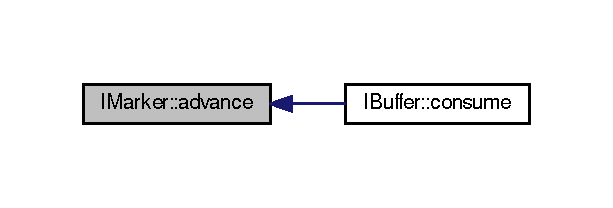
\includegraphics[width=296pt]{class_i_marker_a68c539e79c3052ba7addf090dfd05985_icgraph}
\end{center}
\end{figure}


\hypertarget{class_i_marker_ae6fda228fa071a9720e7d2309d47ac6e}{
\index{IMarker@{IMarker}!isMarked@{isMarked}}
\index{isMarked@{isMarked}!IMarker@{IMarker}}
\subsubsection[{isMarked}]{\setlength{\rightskip}{0pt plus 5cm}bool IMarker::isMarked (
\begin{DoxyParamCaption}
\item[{void}]{}
\end{DoxyParamCaption}
)}}
\label{class_i_marker_ae6fda228fa071a9720e7d2309d47ac6e}


Definition at line 45 of file imarker.cpp.



Here is the caller graph for this function:\nopagebreak
\begin{figure}[H]
\begin{center}
\leavevmode
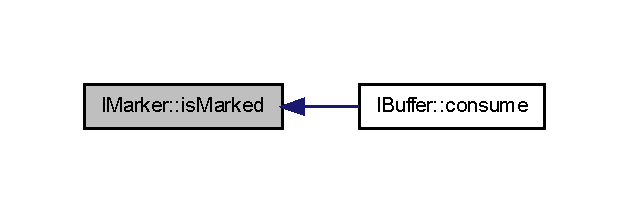
\includegraphics[width=302pt]{class_i_marker_ae6fda228fa071a9720e7d2309d47ac6e_icgraph}
\end{center}
\end{figure}


\hypertarget{class_i_marker_a0e9628e8c66b493ff331abab55c744da}{
\index{IMarker@{IMarker}!location@{location}}
\index{location@{location}!IMarker@{IMarker}}
\subsubsection[{location}]{\setlength{\rightskip}{0pt plus 5cm}unsigned int IMarker::location (
\begin{DoxyParamCaption}
\item[{void}]{}
\end{DoxyParamCaption}
)}}
\label{class_i_marker_a0e9628e8c66b493ff331abab55c744da}


Definition at line 16 of file imarker.cpp.



Here is the caller graph for this function:\nopagebreak
\begin{figure}[H]
\begin{center}
\leavevmode
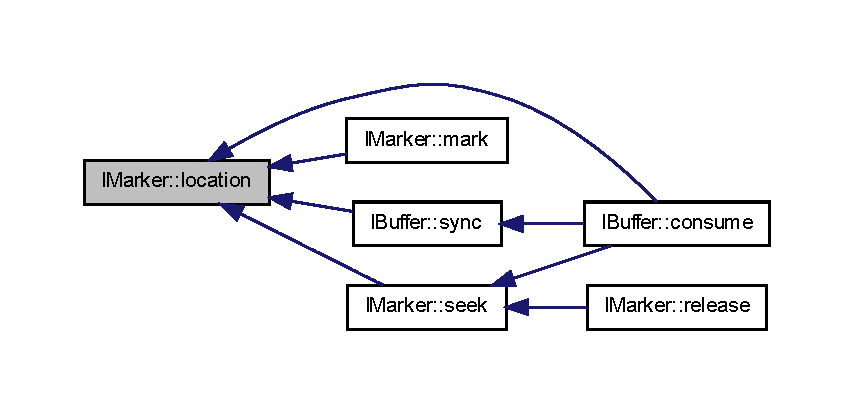
\includegraphics[width=400pt]{class_i_marker_a0e9628e8c66b493ff331abab55c744da_icgraph}
\end{center}
\end{figure}


\hypertarget{class_i_marker_ac2d7a0e8bbfb213378f7a19b50ec9686}{
\index{IMarker@{IMarker}!location@{location}}
\index{location@{location}!IMarker@{IMarker}}
\subsubsection[{location}]{\setlength{\rightskip}{0pt plus 5cm}void IMarker::location (
\begin{DoxyParamCaption}
\item[{unsigned int}]{index}
\end{DoxyParamCaption}
)}}
\label{class_i_marker_ac2d7a0e8bbfb213378f7a19b50ec9686}


Definition at line 21 of file imarker.cpp.

\hypertarget{class_i_marker_a92024922612faa5bb0106609f151c050}{
\index{IMarker@{IMarker}!mark@{mark}}
\index{mark@{mark}!IMarker@{IMarker}}
\subsubsection[{mark}]{\setlength{\rightskip}{0pt plus 5cm}unsigned int IMarker::mark (
\begin{DoxyParamCaption}
\item[{void}]{}
\end{DoxyParamCaption}
)}}
\label{class_i_marker_a92024922612faa5bb0106609f151c050}


Definition at line 26 of file imarker.cpp.



Here is the call graph for this function:\nopagebreak
\begin{figure}[H]
\begin{center}
\leavevmode
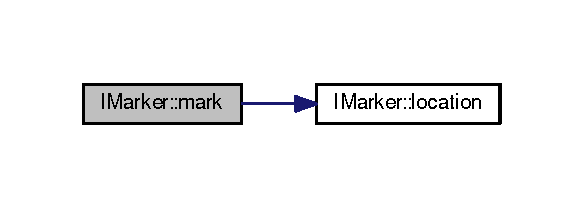
\includegraphics[width=284pt]{class_i_marker_a92024922612faa5bb0106609f151c050_cgraph}
\end{center}
\end{figure}


\hypertarget{class_i_marker_afce4bb0bef01b4579db97e1ca5e64001}{
\index{IMarker@{IMarker}!release@{release}}
\index{release@{release}!IMarker@{IMarker}}
\subsubsection[{release}]{\setlength{\rightskip}{0pt plus 5cm}void IMarker::release (
\begin{DoxyParamCaption}
\item[{void}]{}
\end{DoxyParamCaption}
)}}
\label{class_i_marker_afce4bb0bef01b4579db97e1ca5e64001}


Definition at line 33 of file imarker.cpp.



Here is the call graph for this function:\nopagebreak
\begin{figure}[H]
\begin{center}
\leavevmode
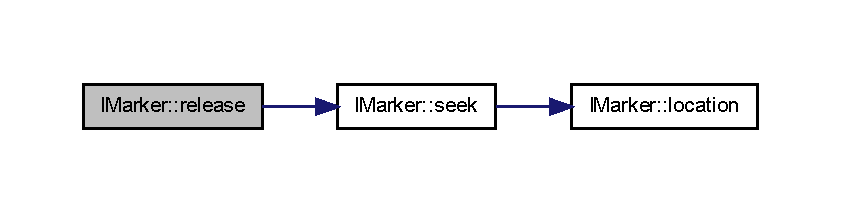
\includegraphics[width=400pt]{class_i_marker_afce4bb0bef01b4579db97e1ca5e64001_cgraph}
\end{center}
\end{figure}


\hypertarget{class_i_marker_a58086bbf091c5b49c15464a070fec171}{
\index{IMarker@{IMarker}!seek@{seek}}
\index{seek@{seek}!IMarker@{IMarker}}
\subsubsection[{seek}]{\setlength{\rightskip}{0pt plus 5cm}void IMarker::seek (
\begin{DoxyParamCaption}
\item[{unsigned int}]{index}
\end{DoxyParamCaption}
)}}
\label{class_i_marker_a58086bbf091c5b49c15464a070fec171}


Definition at line 40 of file imarker.cpp.



Here is the call graph for this function:\nopagebreak
\begin{figure}[H]
\begin{center}
\leavevmode
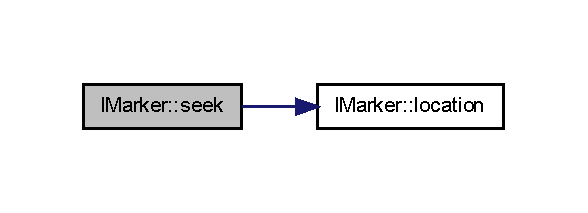
\includegraphics[width=282pt]{class_i_marker_a58086bbf091c5b49c15464a070fec171_cgraph}
\end{center}
\end{figure}




Here is the caller graph for this function:\nopagebreak
\begin{figure}[H]
\begin{center}
\leavevmode
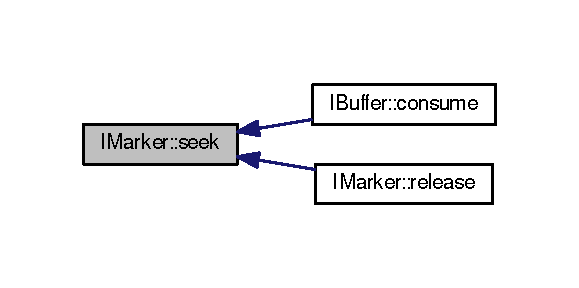
\includegraphics[width=282pt]{class_i_marker_a58086bbf091c5b49c15464a070fec171_icgraph}
\end{center}
\end{figure}




\subsection{Member Data Documentation}
\hypertarget{class_i_marker_adedaefcf6a1b1eac3d728a9d318dc618}{
\index{IMarker@{IMarker}!cur\_\-location@{cur\_\-location}}
\index{cur\_\-location@{cur\_\-location}!IMarker@{IMarker}}
\subsubsection[{cur\_\-location}]{\setlength{\rightskip}{0pt plus 5cm}unsigned int {\bf IMarker::cur\_\-location}\hspace{0.3cm}{\ttfamily  \mbox{[}protected\mbox{]}}}}
\label{class_i_marker_adedaefcf6a1b1eac3d728a9d318dc618}


Definition at line 9 of file imarker.h.

\hypertarget{class_i_marker_a1c1b6ba790e3adf5fa8d9b24c06b10d7}{
\index{IMarker@{IMarker}!markers@{markers}}
\index{markers@{markers}!IMarker@{IMarker}}
\subsubsection[{markers}]{\setlength{\rightskip}{0pt plus 5cm}std::vector$<$unsigned int$>$ {\bf IMarker::markers}\hspace{0.3cm}{\ttfamily  \mbox{[}protected\mbox{]}}}}
\label{class_i_marker_a1c1b6ba790e3adf5fa8d9b24c06b10d7}


Definition at line 10 of file imarker.h.



The documentation for this class was generated from the following files:\begin{DoxyCompactItemize}
\item 
source/marker/\hyperlink{imarker_8h}{imarker.h}\item 
source/marker/\hyperlink{imarker_8cpp}{imarker.cpp}\end{DoxyCompactItemize}

\hypertarget{class_i_parser}{
\section{IParser Class Reference}
\label{class_i_parser}\index{IParser@{IParser}}
}


{\ttfamily \#include $<$iparser.h$>$}



Inheritance diagram for IParser:\nopagebreak
\begin{figure}[H]
\begin{center}
\leavevmode
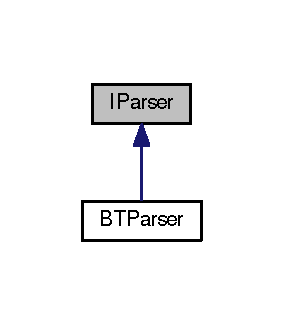
\includegraphics[width=216pt]{class_i_parser__inherit__graph}
\end{center}
\end{figure}


Collaboration diagram for IParser:\nopagebreak
\begin{figure}[H]
\begin{center}
\leavevmode
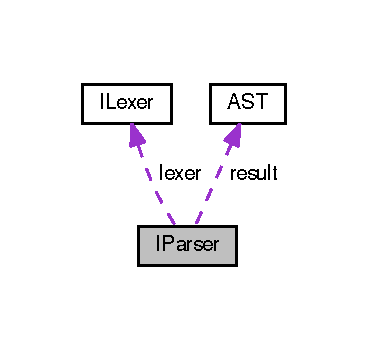
\includegraphics[width=174pt]{class_i_parser__coll__graph}
\end{center}
\end{figure}
\subsection*{Public Member Functions}
\begin{DoxyCompactItemize}
\item 
\hyperlink{class_i_parser_a97691dca898e799fac489ede2ff058b4}{IParser} ()
\item 
\hyperlink{class_i_parser_a7e843f2ae69a52cbacf5bd7b5b9622cf}{IParser} (\hyperlink{class_i_lexer}{ILexer} $\ast$in)
\item 
virtual \hyperlink{class_i_parser_a5b617df0a65b13e5f4be40d764a8ba3b}{$\sim$IParser} ()
\item 
virtual void \hyperlink{class_i_parser_a03bdae30f9a5acb2b9ec5aebb20cc0c2}{parse} ()=0
\item 
virtual void \hyperlink{class_i_parser_a0bb117afecf63b3f2d95b598b763fec2}{input} (\hyperlink{class_i_lexer}{ILexer} $\ast$in)
\item 
virtual const \hyperlink{class_a_s_t}{AST} $\ast$ \hyperlink{class_i_parser_a486e53606cbc75b8a44cfea335ac9c87}{ast} () const 
\item 
virtual void \hyperlink{class_i_parser_ab6b8bb5a97c0bce976135dc4eccc1452}{process} (\hyperlink{class_i_visitor}{IVisitor} \&visitor)
\end{DoxyCompactItemize}
\subsection*{Protected Attributes}
\begin{DoxyCompactItemize}
\item 
\hyperlink{class_a_s_t}{AST} $\ast$ \hyperlink{class_i_parser_a525c62c560492ef3bdb1a21c4da13e04}{result}
\item 
\hyperlink{class_i_lexer}{ILexer} $\ast$ \hyperlink{class_i_parser_a2c89fe9ae1c200eda69c78f7441dea00}{lexer}
\end{DoxyCompactItemize}


\subsection{Detailed Description}


Definition at line 26 of file iparser.h.



\subsection{Constructor \& Destructor Documentation}
\hypertarget{class_i_parser_a97691dca898e799fac489ede2ff058b4}{
\index{IParser@{IParser}!IParser@{IParser}}
\index{IParser@{IParser}!IParser@{IParser}}
\subsubsection[{IParser}]{\setlength{\rightskip}{0pt plus 5cm}IParser::IParser (
\begin{DoxyParamCaption}
{}
\end{DoxyParamCaption}
)}}
\label{class_i_parser_a97691dca898e799fac489ede2ff058b4}


Definition at line 28 of file iparser.cpp.

\hypertarget{class_i_parser_a7e843f2ae69a52cbacf5bd7b5b9622cf}{
\index{IParser@{IParser}!IParser@{IParser}}
\index{IParser@{IParser}!IParser@{IParser}}
\subsubsection[{IParser}]{\setlength{\rightskip}{0pt plus 5cm}IParser::IParser (
\begin{DoxyParamCaption}
\item[{{\bf ILexer} $\ast$}]{in}
\end{DoxyParamCaption}
)}}
\label{class_i_parser_a7e843f2ae69a52cbacf5bd7b5b9622cf}


Definition at line 32 of file iparser.cpp.

\hypertarget{class_i_parser_a5b617df0a65b13e5f4be40d764a8ba3b}{
\index{IParser@{IParser}!$\sim$IParser@{$\sim$IParser}}
\index{$\sim$IParser@{$\sim$IParser}!IParser@{IParser}}
\subsubsection[{$\sim$IParser}]{\setlength{\rightskip}{0pt plus 5cm}IParser::$\sim$IParser (
\begin{DoxyParamCaption}
{}
\end{DoxyParamCaption}
)\hspace{0.3cm}{\ttfamily  \mbox{[}virtual\mbox{]}}}}
\label{class_i_parser_a5b617df0a65b13e5f4be40d764a8ba3b}


Definition at line 36 of file iparser.cpp.



\subsection{Member Function Documentation}
\hypertarget{class_i_parser_a486e53606cbc75b8a44cfea335ac9c87}{
\index{IParser@{IParser}!ast@{ast}}
\index{ast@{ast}!IParser@{IParser}}
\subsubsection[{ast}]{\setlength{\rightskip}{0pt plus 5cm}const {\bf AST} $\ast$ IParser::ast (
\begin{DoxyParamCaption}
{}
\end{DoxyParamCaption}
) const\hspace{0.3cm}{\ttfamily  \mbox{[}virtual\mbox{]}}}}
\label{class_i_parser_a486e53606cbc75b8a44cfea335ac9c87}


Definition at line 54 of file iparser.cpp.

\hypertarget{class_i_parser_a0bb117afecf63b3f2d95b598b763fec2}{
\index{IParser@{IParser}!input@{input}}
\index{input@{input}!IParser@{IParser}}
\subsubsection[{input}]{\setlength{\rightskip}{0pt plus 5cm}void IParser::input (
\begin{DoxyParamCaption}
\item[{{\bf ILexer} $\ast$}]{in}
\end{DoxyParamCaption}
)\hspace{0.3cm}{\ttfamily  \mbox{[}virtual\mbox{]}}}}
\label{class_i_parser_a0bb117afecf63b3f2d95b598b763fec2}


Definition at line 49 of file iparser.cpp.

\hypertarget{class_i_parser_a03bdae30f9a5acb2b9ec5aebb20cc0c2}{
\index{IParser@{IParser}!parse@{parse}}
\index{parse@{parse}!IParser@{IParser}}
\subsubsection[{parse}]{\setlength{\rightskip}{0pt plus 5cm}virtual void IParser::parse (
\begin{DoxyParamCaption}
{}
\end{DoxyParamCaption}
)\hspace{0.3cm}{\ttfamily  \mbox{[}pure virtual\mbox{]}}}}
\label{class_i_parser_a03bdae30f9a5acb2b9ec5aebb20cc0c2}
\hypertarget{class_i_parser_ab6b8bb5a97c0bce976135dc4eccc1452}{
\index{IParser@{IParser}!process@{process}}
\index{process@{process}!IParser@{IParser}}
\subsubsection[{process}]{\setlength{\rightskip}{0pt plus 5cm}void IParser::process (
\begin{DoxyParamCaption}
\item[{{\bf IVisitor} \&}]{visitor}
\end{DoxyParamCaption}
)\hspace{0.3cm}{\ttfamily  \mbox{[}virtual\mbox{]}}}}
\label{class_i_parser_ab6b8bb5a97c0bce976135dc4eccc1452}


Definition at line 59 of file iparser.cpp.



Here is the call graph for this function:\nopagebreak
\begin{figure}[H]
\begin{center}
\leavevmode
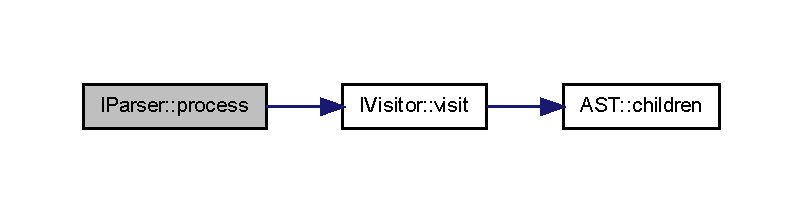
\includegraphics[width=386pt]{class_i_parser_ab6b8bb5a97c0bce976135dc4eccc1452_cgraph}
\end{center}
\end{figure}




\subsection{Member Data Documentation}
\hypertarget{class_i_parser_a2c89fe9ae1c200eda69c78f7441dea00}{
\index{IParser@{IParser}!lexer@{lexer}}
\index{lexer@{lexer}!IParser@{IParser}}
\subsubsection[{lexer}]{\setlength{\rightskip}{0pt plus 5cm}{\bf ILexer}$\ast$ {\bf IParser::lexer}\hspace{0.3cm}{\ttfamily  \mbox{[}protected\mbox{]}}}}
\label{class_i_parser_a2c89fe9ae1c200eda69c78f7441dea00}


Definition at line 29 of file iparser.h.

\hypertarget{class_i_parser_a525c62c560492ef3bdb1a21c4da13e04}{
\index{IParser@{IParser}!result@{result}}
\index{result@{result}!IParser@{IParser}}
\subsubsection[{result}]{\setlength{\rightskip}{0pt plus 5cm}{\bf AST}$\ast$ {\bf IParser::result}\hspace{0.3cm}{\ttfamily  \mbox{[}protected\mbox{]}}}}
\label{class_i_parser_a525c62c560492ef3bdb1a21c4da13e04}


Definition at line 28 of file iparser.h.



The documentation for this class was generated from the following files:\begin{DoxyCompactItemize}
\item 
source/parser/\hyperlink{iparser_8h}{iparser.h}\item 
source/parser/\hyperlink{iparser_8cpp}{iparser.cpp}\end{DoxyCompactItemize}

\hypertarget{class_i_visitor}{
\section{IVisitor Class Reference}
\label{class_i_visitor}\index{IVisitor@{IVisitor}}
}


{\ttfamily \#include $<$ivisitor.h$>$}



Inheritance diagram for IVisitor:
\nopagebreak
\begin{figure}[H]
\begin{center}
\leavevmode
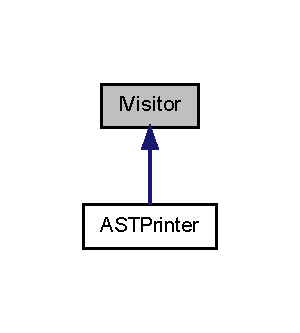
\includegraphics[width=144pt]{class_i_visitor__inherit__graph}
\end{center}
\end{figure}
\subsection*{Public Member Functions}
\begin{DoxyCompactItemize}
\item 
\hyperlink{class_i_visitor_a1f982003291f872f6f3781456b295e8a}{IVisitor} ()
\item 
\hyperlink{class_i_visitor_a05534ba3ad2710875aa918c3d917a088}{$\sim$IVisitor} ()
\item 
void \hyperlink{class_i_visitor_ae1fa19302cb2c14a8e98094cb3e990f4}{visit} (\hyperlink{class_a_s_t}{AST} $\ast$cur, int depth=0)
\end{DoxyCompactItemize}


\subsection{Detailed Description}


Definition at line 8 of file ivisitor.h.



\subsection{Constructor \& Destructor Documentation}
\hypertarget{class_i_visitor_a1f982003291f872f6f3781456b295e8a}{
\index{IVisitor@{IVisitor}!IVisitor@{IVisitor}}
\index{IVisitor@{IVisitor}!IVisitor@{IVisitor}}
\subsubsection[{IVisitor}]{\setlength{\rightskip}{0pt plus 5cm}IVisitor::IVisitor (
\begin{DoxyParamCaption}
{}
\end{DoxyParamCaption}
)}}
\label{class_i_visitor_a1f982003291f872f6f3781456b295e8a}


Definition at line 6 of file ivisitor.cpp.

\hypertarget{class_i_visitor_a05534ba3ad2710875aa918c3d917a088}{
\index{IVisitor@{IVisitor}!$\sim$IVisitor@{$\sim$IVisitor}}
\index{$\sim$IVisitor@{$\sim$IVisitor}!IVisitor@{IVisitor}}
\subsubsection[{$\sim$IVisitor}]{\setlength{\rightskip}{0pt plus 5cm}IVisitor::$\sim$IVisitor (
\begin{DoxyParamCaption}
{}
\end{DoxyParamCaption}
)}}
\label{class_i_visitor_a05534ba3ad2710875aa918c3d917a088}


Definition at line 10 of file ivisitor.cpp.



\subsection{Member Function Documentation}
\hypertarget{class_i_visitor_ae1fa19302cb2c14a8e98094cb3e990f4}{
\index{IVisitor@{IVisitor}!visit@{visit}}
\index{visit@{visit}!IVisitor@{IVisitor}}
\subsubsection[{visit}]{\setlength{\rightskip}{0pt plus 5cm}void IVisitor::visit (
\begin{DoxyParamCaption}
\item[{{\bf AST} $\ast$}]{cur, }
\item[{int}]{depth = {\ttfamily 0}}
\end{DoxyParamCaption}
)}}
\label{class_i_visitor_ae1fa19302cb2c14a8e98094cb3e990f4}


Definition at line 14 of file ivisitor.cpp.



Here is the call graph for this function:
\nopagebreak
\begin{figure}[H]
\begin{center}
\leavevmode
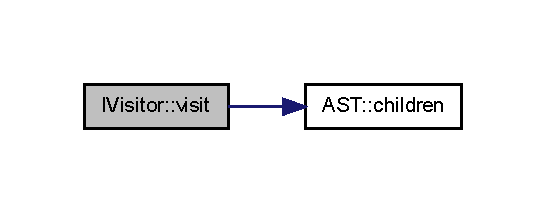
\includegraphics[width=262pt]{class_i_visitor_ae1fa19302cb2c14a8e98094cb3e990f4_cgraph}
\end{center}
\end{figure}




Here is the caller graph for this function:
\nopagebreak
\begin{figure}[H]
\begin{center}
\leavevmode
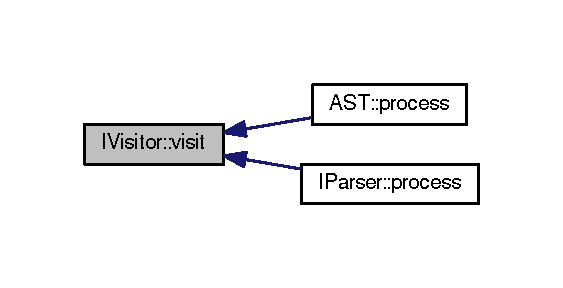
\includegraphics[width=274pt]{class_i_visitor_ae1fa19302cb2c14a8e98094cb3e990f4_icgraph}
\end{center}
\end{figure}




The documentation for this class was generated from the following files:\begin{DoxyCompactItemize}
\item 
source/visitor/\hyperlink{ivisitor_8h}{ivisitor.h}\item 
source/visitor/\hyperlink{ivisitor_8cpp}{ivisitor.cpp}\end{DoxyCompactItemize}

\hypertarget{class_l_l_k_parser}{
\section{LLKParser Class Reference}
\label{class_l_l_k_parser}\index{LLKParser@{LLKParser}}
}


{\ttfamily \#include $<$llkparser.h$>$}



Inheritance diagram for LLKParser:
\nopagebreak
\begin{figure}[H]
\begin{center}
\leavevmode
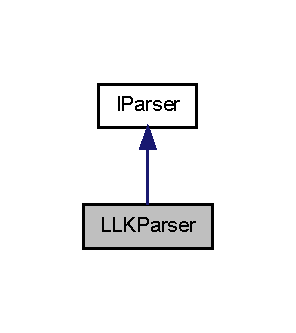
\includegraphics[width=142pt]{class_l_l_k_parser__inherit__graph}
\end{center}
\end{figure}


Collaboration diagram for LLKParser:
\nopagebreak
\begin{figure}[H]
\begin{center}
\leavevmode
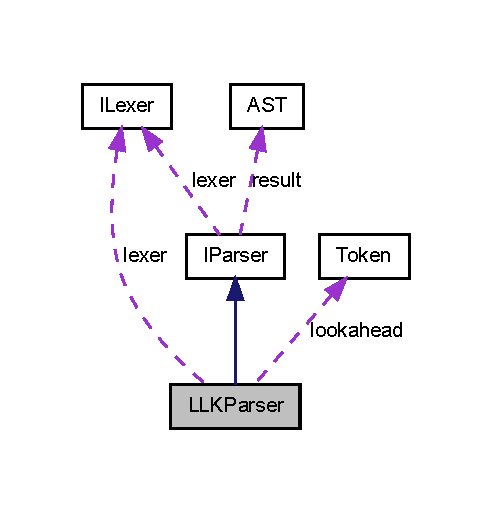
\includegraphics[width=236pt]{class_l_l_k_parser__coll__graph}
\end{center}
\end{figure}
\subsection*{Public Member Functions}
\begin{DoxyCompactItemize}
\item 
\hyperlink{class_l_l_k_parser_ac7ef031af84926f26f30a7c19030014c}{LLKParser} (int k\_\-val, \hyperlink{class_i_lexer}{ILexer} $\ast$lxer)
\item 
\hyperlink{class_l_l_k_parser_a3955a407d454fdfddb86e578250c9205}{$\sim$LLKParser} ()
\item 
void \hyperlink{class_l_l_k_parser_acbea9850c2fe482395af42e5fc05f2fa}{consume} (void)
\item 
void \hyperlink{class_l_l_k_parser_adefd01a8ab2f64530cf3918fc74885a6}{match} (\hyperlink{token_8h_abf05bcc4c1b09928131e6afd3b768a77}{TokenType\_\-T} type)
\item 
\hyperlink{class_token}{Token} \& \hyperlink{class_l_l_k_parser_aa5fdc66d3c8f97498b77950bda4078e4}{lookaheadToken} (int i)
\item 
\hyperlink{token_8h_abf05bcc4c1b09928131e6afd3b768a77}{TokenType\_\-T} \hyperlink{class_l_l_k_parser_affcd736d86542ea9c890bc59a46c8ddf}{lookaheadType} (int i)
\end{DoxyCompactItemize}


\subsection{Detailed Description}


Definition at line 9 of file llkparser.h.



\subsection{Constructor \& Destructor Documentation}
\hypertarget{class_l_l_k_parser_ac7ef031af84926f26f30a7c19030014c}{
\index{LLKParser@{LLKParser}!LLKParser@{LLKParser}}
\index{LLKParser@{LLKParser}!LLKParser@{LLKParser}}
\subsubsection[{LLKParser}]{\setlength{\rightskip}{0pt plus 5cm}LLKParser::LLKParser (
\begin{DoxyParamCaption}
\item[{int}]{k\_\-val, }
\item[{{\bf ILexer} $\ast$}]{lxer}
\end{DoxyParamCaption}
)}}
\label{class_l_l_k_parser_ac7ef031af84926f26f30a7c19030014c}


Definition at line 4 of file llkparser.cpp.

\hypertarget{class_l_l_k_parser_a3955a407d454fdfddb86e578250c9205}{
\index{LLKParser@{LLKParser}!$\sim$LLKParser@{$\sim$LLKParser}}
\index{$\sim$LLKParser@{$\sim$LLKParser}!LLKParser@{LLKParser}}
\subsubsection[{$\sim$LLKParser}]{\setlength{\rightskip}{0pt plus 5cm}LLKParser::$\sim$LLKParser (
\begin{DoxyParamCaption}
{}
\end{DoxyParamCaption}
)}}
\label{class_l_l_k_parser_a3955a407d454fdfddb86e578250c9205}


Definition at line 18 of file llkparser.cpp.



\subsection{Member Function Documentation}
\hypertarget{class_l_l_k_parser_acbea9850c2fe482395af42e5fc05f2fa}{
\index{LLKParser@{LLKParser}!consume@{consume}}
\index{consume@{consume}!LLKParser@{LLKParser}}
\subsubsection[{consume}]{\setlength{\rightskip}{0pt plus 5cm}void LLKParser::consume (
\begin{DoxyParamCaption}
\item[{void}]{}
\end{DoxyParamCaption}
)}}
\label{class_l_l_k_parser_acbea9850c2fe482395af42e5fc05f2fa}


Definition at line 26 of file llkparser.cpp.



Here is the call graph for this function:
\nopagebreak
\begin{figure}[H]
\begin{center}
\leavevmode
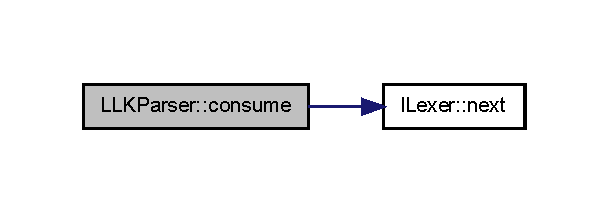
\includegraphics[width=292pt]{class_l_l_k_parser_acbea9850c2fe482395af42e5fc05f2fa_cgraph}
\end{center}
\end{figure}




Here is the caller graph for this function:
\nopagebreak
\begin{figure}[H]
\begin{center}
\leavevmode
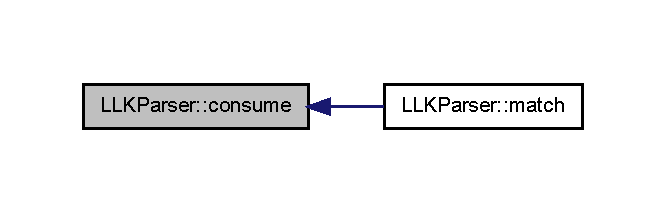
\includegraphics[width=320pt]{class_l_l_k_parser_acbea9850c2fe482395af42e5fc05f2fa_icgraph}
\end{center}
\end{figure}


\hypertarget{class_l_l_k_parser_aa5fdc66d3c8f97498b77950bda4078e4}{
\index{LLKParser@{LLKParser}!lookaheadToken@{lookaheadToken}}
\index{lookaheadToken@{lookaheadToken}!LLKParser@{LLKParser}}
\subsubsection[{lookaheadToken}]{\setlength{\rightskip}{0pt plus 5cm}{\bf Token} \& LLKParser::lookaheadToken (
\begin{DoxyParamCaption}
\item[{int}]{i}
\end{DoxyParamCaption}
)}}
\label{class_l_l_k_parser_aa5fdc66d3c8f97498b77950bda4078e4}


Definition at line 49 of file llkparser.cpp.



Here is the caller graph for this function:
\nopagebreak
\begin{figure}[H]
\begin{center}
\leavevmode
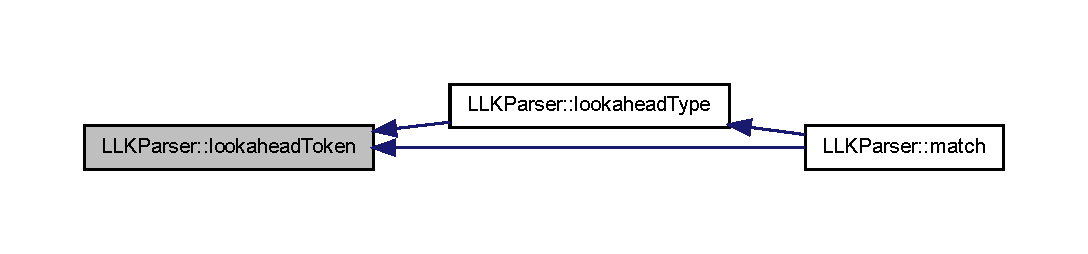
\includegraphics[width=400pt]{class_l_l_k_parser_aa5fdc66d3c8f97498b77950bda4078e4_icgraph}
\end{center}
\end{figure}


\hypertarget{class_l_l_k_parser_affcd736d86542ea9c890bc59a46c8ddf}{
\index{LLKParser@{LLKParser}!lookaheadType@{lookaheadType}}
\index{lookaheadType@{lookaheadType}!LLKParser@{LLKParser}}
\subsubsection[{lookaheadType}]{\setlength{\rightskip}{0pt plus 5cm}{\bf TokenType\_\-T} LLKParser::lookaheadType (
\begin{DoxyParamCaption}
\item[{int}]{i}
\end{DoxyParamCaption}
)}}
\label{class_l_l_k_parser_affcd736d86542ea9c890bc59a46c8ddf}


Definition at line 55 of file llkparser.cpp.



Here is the call graph for this function:
\nopagebreak
\begin{figure}[H]
\begin{center}
\leavevmode
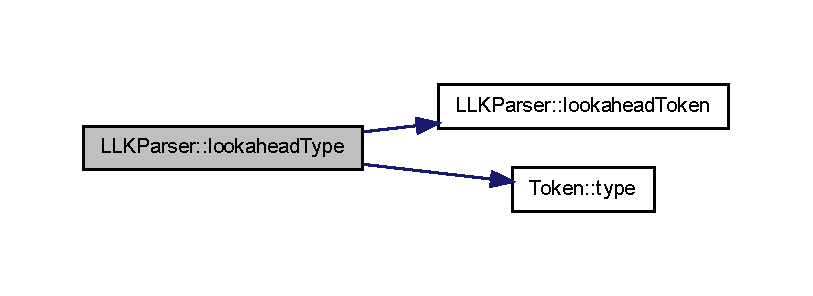
\includegraphics[width=390pt]{class_l_l_k_parser_affcd736d86542ea9c890bc59a46c8ddf_cgraph}
\end{center}
\end{figure}




Here is the caller graph for this function:
\nopagebreak
\begin{figure}[H]
\begin{center}
\leavevmode
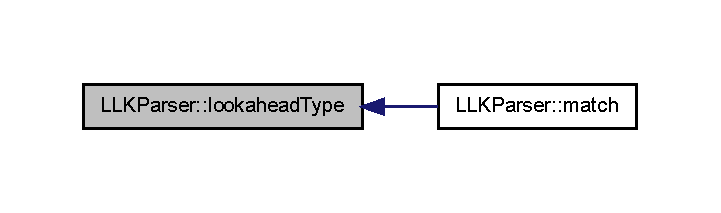
\includegraphics[width=346pt]{class_l_l_k_parser_affcd736d86542ea9c890bc59a46c8ddf_icgraph}
\end{center}
\end{figure}


\hypertarget{class_l_l_k_parser_adefd01a8ab2f64530cf3918fc74885a6}{
\index{LLKParser@{LLKParser}!match@{match}}
\index{match@{match}!LLKParser@{LLKParser}}
\subsubsection[{match}]{\setlength{\rightskip}{0pt plus 5cm}void LLKParser::match (
\begin{DoxyParamCaption}
\item[{{\bf TokenType\_\-T}}]{type}
\end{DoxyParamCaption}
)}}
\label{class_l_l_k_parser_adefd01a8ab2f64530cf3918fc74885a6}


Definition at line 35 of file llkparser.cpp.



Here is the call graph for this function:
\nopagebreak
\begin{figure}[H]
\begin{center}
\leavevmode
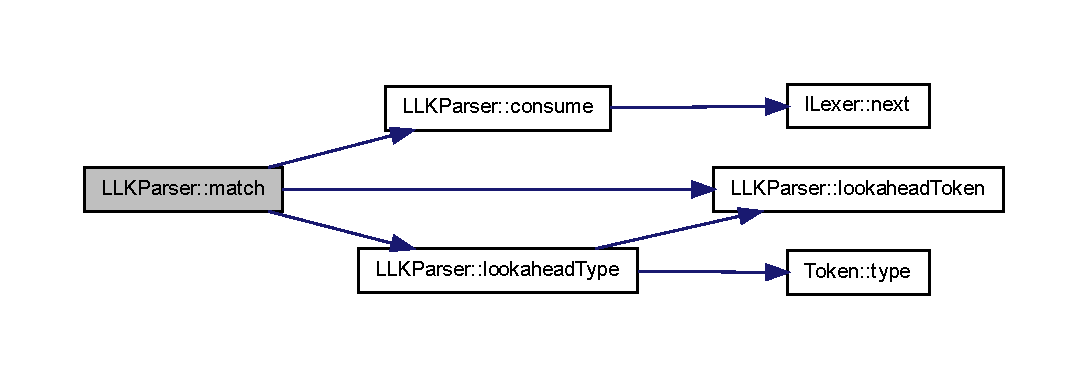
\includegraphics[width=400pt]{class_l_l_k_parser_adefd01a8ab2f64530cf3918fc74885a6_cgraph}
\end{center}
\end{figure}




The documentation for this class was generated from the following files:\begin{DoxyCompactItemize}
\item 
source/parser/llkparser/\hyperlink{llkparser_8h}{llkparser.h}\item 
source/parser/llkparser/\hyperlink{llkparser_8cpp}{llkparser.cpp}\end{DoxyCompactItemize}

\hypertarget{class_l_l_n_lexer}{\section{L\-L\-N\-Lexer Class Reference}
\label{class_l_l_n_lexer}\index{L\-L\-N\-Lexer@{L\-L\-N\-Lexer}}
}


{\ttfamily \#include $<$llnlexer.\-h$>$}



Inheritance diagram for L\-L\-N\-Lexer\-:
\nopagebreak
\begin{figure}[H]
\begin{center}
\leavevmode
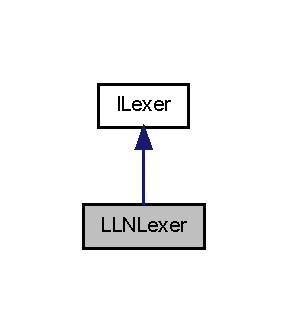
\includegraphics[width=136pt]{class_l_l_n_lexer__inherit__graph}
\end{center}
\end{figure}


Collaboration diagram for L\-L\-N\-Lexer\-:
\nopagebreak
\begin{figure}[H]
\begin{center}
\leavevmode
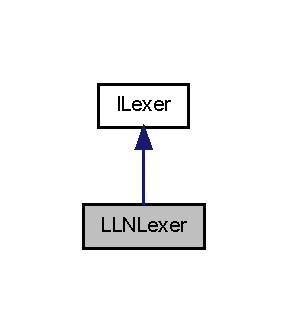
\includegraphics[width=136pt]{class_l_l_n_lexer__coll__graph}
\end{center}
\end{figure}
\subsection*{Public Member Functions}
\begin{DoxyCompactItemize}
\item 
\hyperlink{class_l_l_n_lexer_a80d72ef409a84e097a52ddb6d3cf9843}{L\-L\-N\-Lexer} (std\-::istream \&in)
\item 
virtual \hyperlink{class_l_l_n_lexer_ab4c8e44583f3d144df1379ea4d70b42b}{$\sim$\-L\-L\-N\-Lexer} ()
\item 
void \hyperlink{class_l_l_n_lexer_ada670d39fa588ed793c71fe286ffe01d}{consume} (void)
\item 
void \hyperlink{class_l_l_n_lexer_a4c250c0e032a7cc3e0ffbdcf8c3b18b7}{match} (char type)
\item 
void \hyperlink{class_l_l_n_lexer_a63acbcfa3e703992774a6071a49d1735}{sync} (unsigned int i)
\item 
void \hyperlink{class_l_l_n_lexer_a6a736fa44bf3553a7792d84ab9598eaa}{fill} (unsigned int n)
\item 
char \hyperlink{class_l_l_n_lexer_a66d139156eeb71c9017cfa55acc6ae89}{lookahead} (unsigned int i)
\item 
\hyperlink{class_token}{Token} \hyperlink{class_l_l_n_lexer_a3832522afb32a85b3171f552ff9dd676}{next} (void)=0
\end{DoxyCompactItemize}
\subsection*{Protected Attributes}
\begin{DoxyCompactItemize}
\item 
unsigned int \hyperlink{class_l_l_n_lexer_a6cac67fbdbdc8083f87e1d0938d68ba2}{cur\-\_\-idx}
\item 
std\-::vector$<$ char $>$ \hyperlink{class_l_l_n_lexer_a6e583dda9f354ddb453c277be2cb6edc}{la\-\_\-buffer}
\end{DoxyCompactItemize}


\subsection{Detailed Description}


Definition at line 7 of file llnlexer.\-h.



\subsection{Constructor \& Destructor Documentation}
\hypertarget{class_l_l_n_lexer_a80d72ef409a84e097a52ddb6d3cf9843}{\index{L\-L\-N\-Lexer@{L\-L\-N\-Lexer}!L\-L\-N\-Lexer@{L\-L\-N\-Lexer}}
\index{L\-L\-N\-Lexer@{L\-L\-N\-Lexer}!LLNLexer@{L\-L\-N\-Lexer}}
\subsubsection[{L\-L\-N\-Lexer}]{\setlength{\rightskip}{0pt plus 5cm}L\-L\-N\-Lexer\-::\-L\-L\-N\-Lexer (
\begin{DoxyParamCaption}
\item[{std\-::istream \&}]{in}
\end{DoxyParamCaption}
)}}\label{class_l_l_n_lexer_a80d72ef409a84e097a52ddb6d3cf9843}


Definition at line 4 of file llnlexer.\-cpp.

\hypertarget{class_l_l_n_lexer_ab4c8e44583f3d144df1379ea4d70b42b}{\index{L\-L\-N\-Lexer@{L\-L\-N\-Lexer}!$\sim$\-L\-L\-N\-Lexer@{$\sim$\-L\-L\-N\-Lexer}}
\index{$\sim$\-L\-L\-N\-Lexer@{$\sim$\-L\-L\-N\-Lexer}!LLNLexer@{L\-L\-N\-Lexer}}
\subsubsection[{$\sim$\-L\-L\-N\-Lexer}]{\setlength{\rightskip}{0pt plus 5cm}L\-L\-N\-Lexer\-::$\sim$\-L\-L\-N\-Lexer (
\begin{DoxyParamCaption}
{}
\end{DoxyParamCaption}
)\hspace{0.3cm}{\ttfamily [virtual]}}}\label{class_l_l_n_lexer_ab4c8e44583f3d144df1379ea4d70b42b}


Definition at line 8 of file llnlexer.\-cpp.



\subsection{Member Function Documentation}
\hypertarget{class_l_l_n_lexer_ada670d39fa588ed793c71fe286ffe01d}{\index{L\-L\-N\-Lexer@{L\-L\-N\-Lexer}!consume@{consume}}
\index{consume@{consume}!LLNLexer@{L\-L\-N\-Lexer}}
\subsubsection[{consume}]{\setlength{\rightskip}{0pt plus 5cm}void L\-L\-N\-Lexer\-::consume (
\begin{DoxyParamCaption}
\item[{void}]{}
\end{DoxyParamCaption}
)\hspace{0.3cm}{\ttfamily [virtual]}}}\label{class_l_l_n_lexer_ada670d39fa588ed793c71fe286ffe01d}


Implements \hyperlink{class_i_lexer_ae1009b9b2a1e023e1a7d2fd75806607f}{I\-Lexer}.



Definition at line 12 of file llnlexer.\-cpp.



Here is the call graph for this function\-:
\nopagebreak
\begin{figure}[H]
\begin{center}
\leavevmode
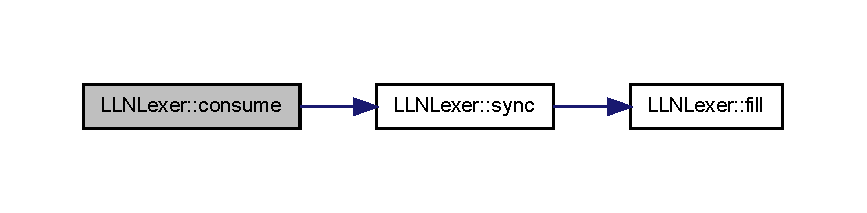
\includegraphics[width=350pt]{class_l_l_n_lexer_ada670d39fa588ed793c71fe286ffe01d_cgraph}
\end{center}
\end{figure}




Here is the caller graph for this function\-:
\nopagebreak
\begin{figure}[H]
\begin{center}
\leavevmode
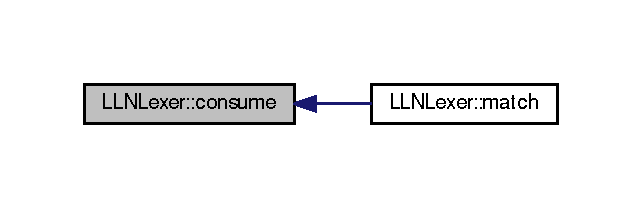
\includegraphics[width=308pt]{class_l_l_n_lexer_ada670d39fa588ed793c71fe286ffe01d_icgraph}
\end{center}
\end{figure}


\hypertarget{class_l_l_n_lexer_a6a736fa44bf3553a7792d84ab9598eaa}{\index{L\-L\-N\-Lexer@{L\-L\-N\-Lexer}!fill@{fill}}
\index{fill@{fill}!LLNLexer@{L\-L\-N\-Lexer}}
\subsubsection[{fill}]{\setlength{\rightskip}{0pt plus 5cm}void L\-L\-N\-Lexer\-::fill (
\begin{DoxyParamCaption}
\item[{unsigned int}]{n}
\end{DoxyParamCaption}
)}}\label{class_l_l_n_lexer_a6a736fa44bf3553a7792d84ab9598eaa}


Definition at line 63 of file llnlexer.\-cpp.



Here is the caller graph for this function\-:
\nopagebreak
\begin{figure}[H]
\begin{center}
\leavevmode
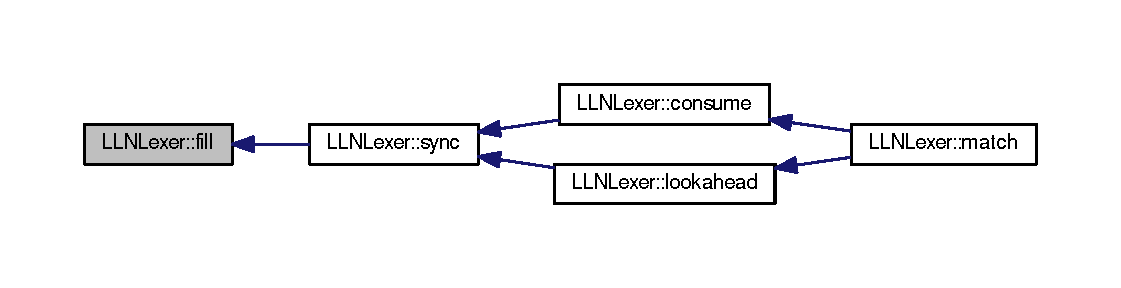
\includegraphics[width=350pt]{class_l_l_n_lexer_a6a736fa44bf3553a7792d84ab9598eaa_icgraph}
\end{center}
\end{figure}


\hypertarget{class_l_l_n_lexer_a66d139156eeb71c9017cfa55acc6ae89}{\index{L\-L\-N\-Lexer@{L\-L\-N\-Lexer}!lookahead@{lookahead}}
\index{lookahead@{lookahead}!LLNLexer@{L\-L\-N\-Lexer}}
\subsubsection[{lookahead}]{\setlength{\rightskip}{0pt plus 5cm}char L\-L\-N\-Lexer\-::lookahead (
\begin{DoxyParamCaption}
\item[{unsigned int}]{i}
\end{DoxyParamCaption}
)}}\label{class_l_l_n_lexer_a66d139156eeb71c9017cfa55acc6ae89}


Definition at line 72 of file llnlexer.\-cpp.



Here is the call graph for this function\-:
\nopagebreak
\begin{figure}[H]
\begin{center}
\leavevmode
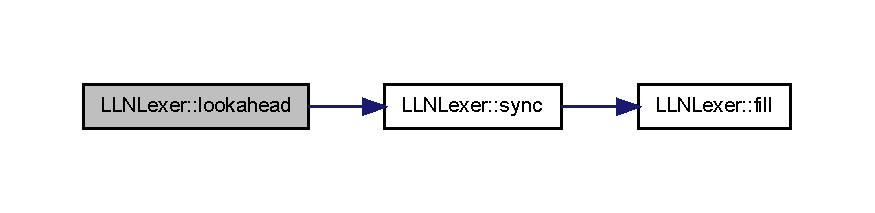
\includegraphics[width=350pt]{class_l_l_n_lexer_a66d139156eeb71c9017cfa55acc6ae89_cgraph}
\end{center}
\end{figure}




Here is the caller graph for this function\-:
\nopagebreak
\begin{figure}[H]
\begin{center}
\leavevmode
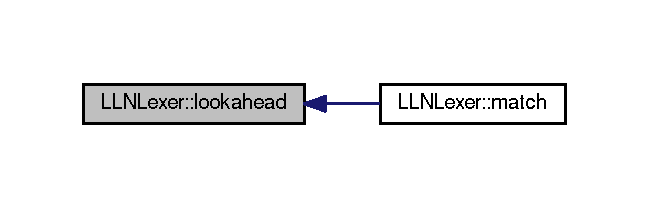
\includegraphics[width=312pt]{class_l_l_n_lexer_a66d139156eeb71c9017cfa55acc6ae89_icgraph}
\end{center}
\end{figure}


\hypertarget{class_l_l_n_lexer_a4c250c0e032a7cc3e0ffbdcf8c3b18b7}{\index{L\-L\-N\-Lexer@{L\-L\-N\-Lexer}!match@{match}}
\index{match@{match}!LLNLexer@{L\-L\-N\-Lexer}}
\subsubsection[{match}]{\setlength{\rightskip}{0pt plus 5cm}void L\-L\-N\-Lexer\-::match (
\begin{DoxyParamCaption}
\item[{char}]{type}
\end{DoxyParamCaption}
)\hspace{0.3cm}{\ttfamily [virtual]}}}\label{class_l_l_n_lexer_a4c250c0e032a7cc3e0ffbdcf8c3b18b7}


Implements \hyperlink{class_i_lexer_a556fdc7b13486f03cb7c3d7d4612666c}{I\-Lexer}.



Definition at line 34 of file llnlexer.\-cpp.



Here is the call graph for this function\-:
\nopagebreak
\begin{figure}[H]
\begin{center}
\leavevmode
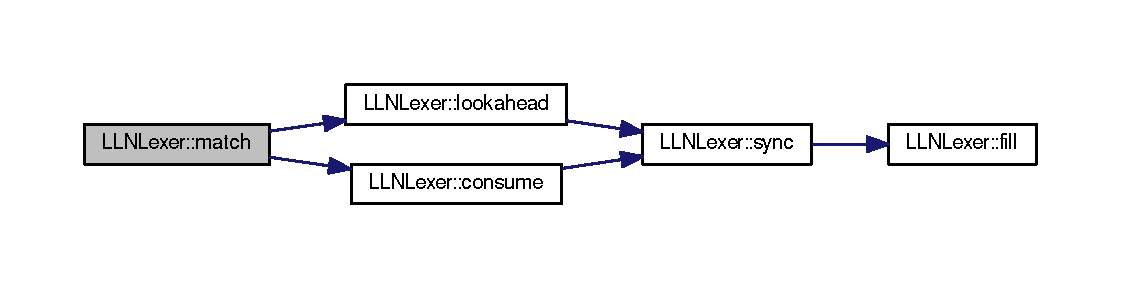
\includegraphics[width=350pt]{class_l_l_n_lexer_a4c250c0e032a7cc3e0ffbdcf8c3b18b7_cgraph}
\end{center}
\end{figure}


\hypertarget{class_l_l_n_lexer_a3832522afb32a85b3171f552ff9dd676}{\index{L\-L\-N\-Lexer@{L\-L\-N\-Lexer}!next@{next}}
\index{next@{next}!LLNLexer@{L\-L\-N\-Lexer}}
\subsubsection[{next}]{\setlength{\rightskip}{0pt plus 5cm}{\bf Token} L\-L\-N\-Lexer\-::next (
\begin{DoxyParamCaption}
\item[{void}]{}
\end{DoxyParamCaption}
)\hspace{0.3cm}{\ttfamily [pure virtual]}}}\label{class_l_l_n_lexer_a3832522afb32a85b3171f552ff9dd676}


Implements \hyperlink{class_i_lexer_a6f5098fda43f68b01d2e7a2a7158c50d}{I\-Lexer}.

\hypertarget{class_l_l_n_lexer_a63acbcfa3e703992774a6071a49d1735}{\index{L\-L\-N\-Lexer@{L\-L\-N\-Lexer}!sync@{sync}}
\index{sync@{sync}!LLNLexer@{L\-L\-N\-Lexer}}
\subsubsection[{sync}]{\setlength{\rightskip}{0pt plus 5cm}void L\-L\-N\-Lexer\-::sync (
\begin{DoxyParamCaption}
\item[{unsigned int}]{i}
\end{DoxyParamCaption}
)}}\label{class_l_l_n_lexer_a63acbcfa3e703992774a6071a49d1735}


Definition at line 48 of file llnlexer.\-cpp.



Here is the call graph for this function\-:
\nopagebreak
\begin{figure}[H]
\begin{center}
\leavevmode
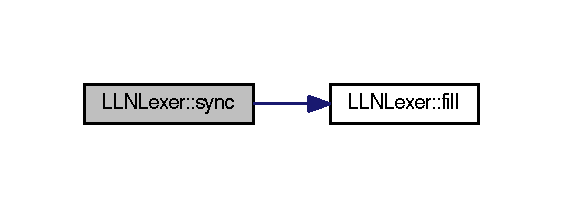
\includegraphics[width=270pt]{class_l_l_n_lexer_a63acbcfa3e703992774a6071a49d1735_cgraph}
\end{center}
\end{figure}




Here is the caller graph for this function\-:
\nopagebreak
\begin{figure}[H]
\begin{center}
\leavevmode
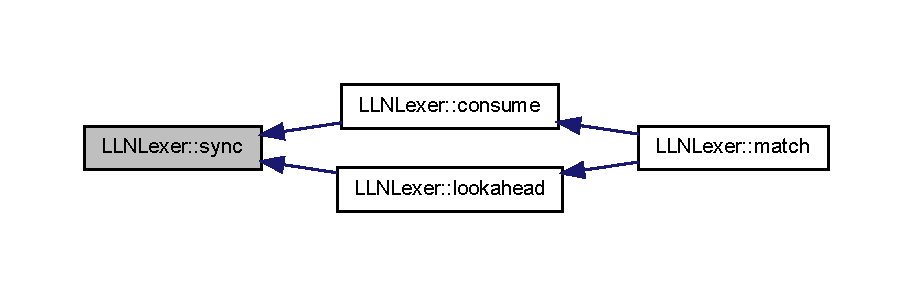
\includegraphics[width=350pt]{class_l_l_n_lexer_a63acbcfa3e703992774a6071a49d1735_icgraph}
\end{center}
\end{figure}




\subsection{Member Data Documentation}
\hypertarget{class_l_l_n_lexer_a6cac67fbdbdc8083f87e1d0938d68ba2}{\index{L\-L\-N\-Lexer@{L\-L\-N\-Lexer}!cur\-\_\-idx@{cur\-\_\-idx}}
\index{cur\-\_\-idx@{cur\-\_\-idx}!LLNLexer@{L\-L\-N\-Lexer}}
\subsubsection[{cur\-\_\-idx}]{\setlength{\rightskip}{0pt plus 5cm}unsigned int L\-L\-N\-Lexer\-::cur\-\_\-idx\hspace{0.3cm}{\ttfamily [protected]}}}\label{class_l_l_n_lexer_a6cac67fbdbdc8083f87e1d0938d68ba2}


Definition at line 10 of file llnlexer.\-h.

\hypertarget{class_l_l_n_lexer_a6e583dda9f354ddb453c277be2cb6edc}{\index{L\-L\-N\-Lexer@{L\-L\-N\-Lexer}!la\-\_\-buffer@{la\-\_\-buffer}}
\index{la\-\_\-buffer@{la\-\_\-buffer}!LLNLexer@{L\-L\-N\-Lexer}}
\subsubsection[{la\-\_\-buffer}]{\setlength{\rightskip}{0pt plus 5cm}std\-::vector$<$char$>$ L\-L\-N\-Lexer\-::la\-\_\-buffer\hspace{0.3cm}{\ttfamily [protected]}}}\label{class_l_l_n_lexer_a6e583dda9f354ddb453c277be2cb6edc}


Definition at line 11 of file llnlexer.\-h.



The documentation for this class was generated from the following files\-:\begin{DoxyCompactItemize}
\item 
source/lexer/llnlexer/\hyperlink{llnlexer_8h}{llnlexer.\-h}\item 
source/lexer/llnlexer/\hyperlink{llnlexer_8cpp}{llnlexer.\-cpp}\end{DoxyCompactItemize}

\hypertarget{class_scope_stack}{
\section{ScopeStack Class Reference}
\label{class_scope_stack}\index{ScopeStack@{ScopeStack}}
}


{\ttfamily \#include $<$scopestack.h$>$}

\subsection*{Public Member Functions}
\begin{DoxyCompactItemize}
\item 
\hyperlink{class_scope_stack_a754459e71e5e91fd4210c063014634c2}{ScopeStack} ()
\item 
virtual \hyperlink{class_scope_stack_a64e2f6ee2758341a649bbbc873b4c626}{$\sim$ScopeStack} ()
\item 
void \hyperlink{class_scope_stack_ae5809bddef2aa253460c1d35ed36c1c8}{startScope} ()
\item 
void \hyperlink{class_scope_stack_a410129444ad5a4be8784007d1fd73129}{stopScope} ()
\item 
void \hyperlink{class_scope_stack_a16f903a19a7223c925d00fe6ba4155f2}{define} (const std::string \&name)
\item 
void \hyperlink{class_scope_stack_ae0c9aa708ebe375e6d4c4eebc4ffc60a}{define} (const std::string \&name, \hyperlink{symbol_8h_a07090a2a79cb68ad8d84e7ecd6558859}{symtype\_\-t} type)
\item 
const \hyperlink{class_symbol}{Symbol} $\ast$ \hyperlink{class_scope_stack_a93cb7113443905f602ba812587e01b4d}{lookup} (const std::string \&name)
\item 
bool \hyperlink{class_scope_stack_a553478b9e13cba1cf77b7f0e7a91c6f4}{isLocal} (const std::string \&name) const 
\item 
bool \hyperlink{class_scope_stack_ae0792790e8cfd148e0cfb67090a790bf}{isGlobal} (const std::string \&name) const 
\end{DoxyCompactItemize}
\subsection*{Protected Attributes}
\begin{DoxyCompactItemize}
\item 
std::list$<$ \hyperlink{scopestack_8h_ac00f2f845911b84646322b4b1c7bc14c}{sym\_\-table\_\-t} $>$ \hyperlink{class_scope_stack_affa1115b1547064c04186846fd594344}{scope\_\-stack}
\end{DoxyCompactItemize}


\subsection{Detailed Description}


Definition at line 12 of file scopestack.h.



\subsection{Constructor \& Destructor Documentation}
\hypertarget{class_scope_stack_a754459e71e5e91fd4210c063014634c2}{
\index{ScopeStack@{ScopeStack}!ScopeStack@{ScopeStack}}
\index{ScopeStack@{ScopeStack}!ScopeStack@{ScopeStack}}
\subsubsection[{ScopeStack}]{\setlength{\rightskip}{0pt plus 5cm}ScopeStack::ScopeStack (
\begin{DoxyParamCaption}
{}
\end{DoxyParamCaption}
)}}
\label{class_scope_stack_a754459e71e5e91fd4210c063014634c2}


Definition at line 6 of file scopestack.cpp.

\hypertarget{class_scope_stack_a64e2f6ee2758341a649bbbc873b4c626}{
\index{ScopeStack@{ScopeStack}!$\sim$ScopeStack@{$\sim$ScopeStack}}
\index{$\sim$ScopeStack@{$\sim$ScopeStack}!ScopeStack@{ScopeStack}}
\subsubsection[{$\sim$ScopeStack}]{\setlength{\rightskip}{0pt plus 5cm}ScopeStack::$\sim$ScopeStack (
\begin{DoxyParamCaption}
{}
\end{DoxyParamCaption}
)\hspace{0.3cm}{\ttfamily  \mbox{[}virtual\mbox{]}}}}
\label{class_scope_stack_a64e2f6ee2758341a649bbbc873b4c626}


Definition at line 13 of file scopestack.cpp.



\subsection{Member Function Documentation}
\hypertarget{class_scope_stack_a16f903a19a7223c925d00fe6ba4155f2}{
\index{ScopeStack@{ScopeStack}!define@{define}}
\index{define@{define}!ScopeStack@{ScopeStack}}
\subsubsection[{define}]{\setlength{\rightskip}{0pt plus 5cm}void ScopeStack::define (
\begin{DoxyParamCaption}
\item[{const std::string \&}]{name}
\end{DoxyParamCaption}
)}}
\label{class_scope_stack_a16f903a19a7223c925d00fe6ba4155f2}


Definition at line 28 of file scopestack.cpp.

\hypertarget{class_scope_stack_ae0c9aa708ebe375e6d4c4eebc4ffc60a}{
\index{ScopeStack@{ScopeStack}!define@{define}}
\index{define@{define}!ScopeStack@{ScopeStack}}
\subsubsection[{define}]{\setlength{\rightskip}{0pt plus 5cm}void ScopeStack::define (
\begin{DoxyParamCaption}
\item[{const std::string \&}]{name, }
\item[{{\bf symtype\_\-t}}]{type}
\end{DoxyParamCaption}
)}}
\label{class_scope_stack_ae0c9aa708ebe375e6d4c4eebc4ffc60a}


Definition at line 34 of file scopestack.cpp.

\hypertarget{class_scope_stack_ae0792790e8cfd148e0cfb67090a790bf}{
\index{ScopeStack@{ScopeStack}!isGlobal@{isGlobal}}
\index{isGlobal@{isGlobal}!ScopeStack@{ScopeStack}}
\subsubsection[{isGlobal}]{\setlength{\rightskip}{0pt plus 5cm}bool ScopeStack::isGlobal (
\begin{DoxyParamCaption}
\item[{const std::string \&}]{name}
\end{DoxyParamCaption}
) const}}
\label{class_scope_stack_ae0792790e8cfd148e0cfb67090a790bf}


Definition at line 66 of file scopestack.cpp.

\hypertarget{class_scope_stack_a553478b9e13cba1cf77b7f0e7a91c6f4}{
\index{ScopeStack@{ScopeStack}!isLocal@{isLocal}}
\index{isLocal@{isLocal}!ScopeStack@{ScopeStack}}
\subsubsection[{isLocal}]{\setlength{\rightskip}{0pt plus 5cm}bool ScopeStack::isLocal (
\begin{DoxyParamCaption}
\item[{const std::string \&}]{name}
\end{DoxyParamCaption}
) const}}
\label{class_scope_stack_a553478b9e13cba1cf77b7f0e7a91c6f4}


Definition at line 55 of file scopestack.cpp.

\hypertarget{class_scope_stack_a93cb7113443905f602ba812587e01b4d}{
\index{ScopeStack@{ScopeStack}!lookup@{lookup}}
\index{lookup@{lookup}!ScopeStack@{ScopeStack}}
\subsubsection[{lookup}]{\setlength{\rightskip}{0pt plus 5cm}const {\bf Symbol} $\ast$ ScopeStack::lookup (
\begin{DoxyParamCaption}
\item[{const std::string \&}]{name}
\end{DoxyParamCaption}
)}}
\label{class_scope_stack_a93cb7113443905f602ba812587e01b4d}


Definition at line 40 of file scopestack.cpp.

\hypertarget{class_scope_stack_ae5809bddef2aa253460c1d35ed36c1c8}{
\index{ScopeStack@{ScopeStack}!startScope@{startScope}}
\index{startScope@{startScope}!ScopeStack@{ScopeStack}}
\subsubsection[{startScope}]{\setlength{\rightskip}{0pt plus 5cm}void ScopeStack::startScope (
\begin{DoxyParamCaption}
{}
\end{DoxyParamCaption}
)}}
\label{class_scope_stack_ae5809bddef2aa253460c1d35ed36c1c8}


Definition at line 17 of file scopestack.cpp.

\hypertarget{class_scope_stack_a410129444ad5a4be8784007d1fd73129}{
\index{ScopeStack@{ScopeStack}!stopScope@{stopScope}}
\index{stopScope@{stopScope}!ScopeStack@{ScopeStack}}
\subsubsection[{stopScope}]{\setlength{\rightskip}{0pt plus 5cm}void ScopeStack::stopScope (
\begin{DoxyParamCaption}
{}
\end{DoxyParamCaption}
)}}
\label{class_scope_stack_a410129444ad5a4be8784007d1fd73129}


Definition at line 23 of file scopestack.cpp.



\subsection{Member Data Documentation}
\hypertarget{class_scope_stack_affa1115b1547064c04186846fd594344}{
\index{ScopeStack@{ScopeStack}!scope\_\-stack@{scope\_\-stack}}
\index{scope\_\-stack@{scope\_\-stack}!ScopeStack@{ScopeStack}}
\subsubsection[{scope\_\-stack}]{\setlength{\rightskip}{0pt plus 5cm}std::list$<${\bf sym\_\-table\_\-t}$>$ {\bf ScopeStack::scope\_\-stack}\hspace{0.3cm}{\ttfamily  \mbox{[}protected\mbox{]}}}}
\label{class_scope_stack_affa1115b1547064c04186846fd594344}


Definition at line 14 of file scopestack.h.



The documentation for this class was generated from the following files:\begin{DoxyCompactItemize}
\item 
source/symbol/\hyperlink{scopestack_8h}{scopestack.h}\item 
source/symbol/\hyperlink{scopestack_8cpp}{scopestack.cpp}\end{DoxyCompactItemize}

\hypertarget{class_symbol}{
\section{Symbol Class Reference}
\label{class_symbol}\index{Symbol@{Symbol}}
}


{\ttfamily \#include $<$symbol.h$>$}

\subsection*{Public Member Functions}
\begin{DoxyCompactItemize}
\item 
\hyperlink{class_symbol_a918bcf3f530e98cc9d97cb16381db88f}{Symbol} (const std::string \&name)
\item 
\hyperlink{class_symbol_a696ddf09a21f1a5a6dacac4e49da076e}{Symbol} (const std::string \&name, \hyperlink{symbol_8h_a07090a2a79cb68ad8d84e7ecd6558859}{symtype\_\-t} type)
\item 
virtual \hyperlink{class_symbol_a505360ad4bd2e0bd1e3954eca1b05723}{$\sim$Symbol} ()
\item 
\hyperlink{symbol_8h_a07090a2a79cb68ad8d84e7ecd6558859}{symtype\_\-t} \hyperlink{class_symbol_afc6ea326ca57f6f9292a05a61f2df362}{type} () const 
\item 
void \hyperlink{class_symbol_a7822b485af2e735d462276836479ff24}{type} (\hyperlink{symbol_8h_a07090a2a79cb68ad8d84e7ecd6558859}{symtype\_\-t} type)
\item 
const std::string \& \hyperlink{class_symbol_a8324a8b8848a9bd1957b8d9e69335112}{name} () const 
\item 
void \hyperlink{class_symbol_a474363d0819a0acf6ecd1a547ec3f926}{name} (const std::string \&name)
\end{DoxyCompactItemize}
\subsection*{Protected Attributes}
\begin{DoxyCompactItemize}
\item 
std::string \hyperlink{class_symbol_a131f02876f25c9bdccbd71e1e7147989}{sym\_\-name}
\item 
\hyperlink{symbol_8h_a07090a2a79cb68ad8d84e7ecd6558859}{symtype\_\-t} \hyperlink{class_symbol_a4cb69009155bb4a73a86fc4004655a31}{sym\_\-type}
\end{DoxyCompactItemize}


\subsection{Detailed Description}


Definition at line 8 of file symbol.h.



\subsection{Constructor \& Destructor Documentation}
\hypertarget{class_symbol_a918bcf3f530e98cc9d97cb16381db88f}{
\index{Symbol@{Symbol}!Symbol@{Symbol}}
\index{Symbol@{Symbol}!Symbol@{Symbol}}
\subsubsection[{Symbol}]{\setlength{\rightskip}{0pt plus 5cm}Symbol::Symbol (
\begin{DoxyParamCaption}
\item[{const std::string \&}]{name}
\end{DoxyParamCaption}
)}}
\label{class_symbol_a918bcf3f530e98cc9d97cb16381db88f}


Definition at line 3 of file symbol.cpp.

\hypertarget{class_symbol_a696ddf09a21f1a5a6dacac4e49da076e}{
\index{Symbol@{Symbol}!Symbol@{Symbol}}
\index{Symbol@{Symbol}!Symbol@{Symbol}}
\subsubsection[{Symbol}]{\setlength{\rightskip}{0pt plus 5cm}Symbol::Symbol (
\begin{DoxyParamCaption}
\item[{const std::string \&}]{name, }
\item[{{\bf symtype\_\-t}}]{type}
\end{DoxyParamCaption}
)}}
\label{class_symbol_a696ddf09a21f1a5a6dacac4e49da076e}


Definition at line 7 of file symbol.cpp.

\hypertarget{class_symbol_a505360ad4bd2e0bd1e3954eca1b05723}{
\index{Symbol@{Symbol}!$\sim$Symbol@{$\sim$Symbol}}
\index{$\sim$Symbol@{$\sim$Symbol}!Symbol@{Symbol}}
\subsubsection[{$\sim$Symbol}]{\setlength{\rightskip}{0pt plus 5cm}Symbol::$\sim$Symbol (
\begin{DoxyParamCaption}
{}
\end{DoxyParamCaption}
)\hspace{0.3cm}{\ttfamily  \mbox{[}virtual\mbox{]}}}}
\label{class_symbol_a505360ad4bd2e0bd1e3954eca1b05723}


Definition at line 11 of file symbol.cpp.



\subsection{Member Function Documentation}
\hypertarget{class_symbol_a8324a8b8848a9bd1957b8d9e69335112}{
\index{Symbol@{Symbol}!name@{name}}
\index{name@{name}!Symbol@{Symbol}}
\subsubsection[{name}]{\setlength{\rightskip}{0pt plus 5cm}const std::string \& Symbol::name (
\begin{DoxyParamCaption}
{}
\end{DoxyParamCaption}
) const}}
\label{class_symbol_a8324a8b8848a9bd1957b8d9e69335112}


Definition at line 25 of file symbol.cpp.



Here is the caller graph for this function:
\nopagebreak
\begin{figure}[H]
\begin{center}
\leavevmode
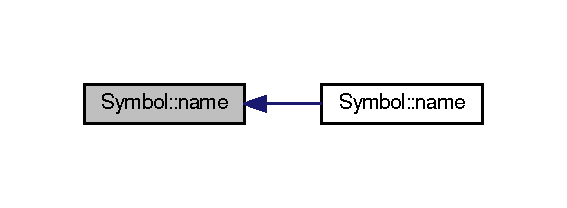
\includegraphics[width=276pt]{class_symbol_a8324a8b8848a9bd1957b8d9e69335112_icgraph}
\end{center}
\end{figure}


\hypertarget{class_symbol_a474363d0819a0acf6ecd1a547ec3f926}{
\index{Symbol@{Symbol}!name@{name}}
\index{name@{name}!Symbol@{Symbol}}
\subsubsection[{name}]{\setlength{\rightskip}{0pt plus 5cm}void Symbol::name (
\begin{DoxyParamCaption}
\item[{const std::string \&}]{name}
\end{DoxyParamCaption}
)}}
\label{class_symbol_a474363d0819a0acf6ecd1a547ec3f926}


Definition at line 30 of file symbol.cpp.



Here is the call graph for this function:
\nopagebreak
\begin{figure}[H]
\begin{center}
\leavevmode
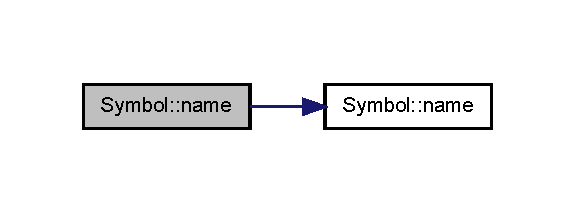
\includegraphics[width=276pt]{class_symbol_a474363d0819a0acf6ecd1a547ec3f926_cgraph}
\end{center}
\end{figure}


\hypertarget{class_symbol_afc6ea326ca57f6f9292a05a61f2df362}{
\index{Symbol@{Symbol}!type@{type}}
\index{type@{type}!Symbol@{Symbol}}
\subsubsection[{type}]{\setlength{\rightskip}{0pt plus 5cm}{\bf symtype\_\-t} Symbol::type (
\begin{DoxyParamCaption}
\item[{void}]{}
\end{DoxyParamCaption}
) const}}
\label{class_symbol_afc6ea326ca57f6f9292a05a61f2df362}


Definition at line 15 of file symbol.cpp.



Here is the caller graph for this function:
\nopagebreak
\begin{figure}[H]
\begin{center}
\leavevmode
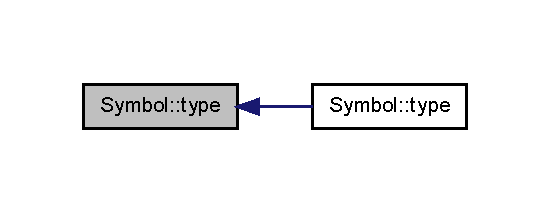
\includegraphics[width=264pt]{class_symbol_afc6ea326ca57f6f9292a05a61f2df362_icgraph}
\end{center}
\end{figure}


\hypertarget{class_symbol_a7822b485af2e735d462276836479ff24}{
\index{Symbol@{Symbol}!type@{type}}
\index{type@{type}!Symbol@{Symbol}}
\subsubsection[{type}]{\setlength{\rightskip}{0pt plus 5cm}void Symbol::type (
\begin{DoxyParamCaption}
\item[{{\bf symtype\_\-t}}]{type}
\end{DoxyParamCaption}
)}}
\label{class_symbol_a7822b485af2e735d462276836479ff24}


Definition at line 20 of file symbol.cpp.



Here is the call graph for this function:
\nopagebreak
\begin{figure}[H]
\begin{center}
\leavevmode
\includegraphics[width=264pt]{class_symbol_a7822b485af2e735d462276836479ff24_cgraph}
\end{center}
\end{figure}




\subsection{Member Data Documentation}
\hypertarget{class_symbol_a131f02876f25c9bdccbd71e1e7147989}{
\index{Symbol@{Symbol}!sym\_\-name@{sym\_\-name}}
\index{sym\_\-name@{sym\_\-name}!Symbol@{Symbol}}
\subsubsection[{sym\_\-name}]{\setlength{\rightskip}{0pt plus 5cm}std::string {\bf Symbol::sym\_\-name}\hspace{0.3cm}{\ttfamily  \mbox{[}protected\mbox{]}}}}
\label{class_symbol_a131f02876f25c9bdccbd71e1e7147989}


Definition at line 10 of file symbol.h.

\hypertarget{class_symbol_a4cb69009155bb4a73a86fc4004655a31}{
\index{Symbol@{Symbol}!sym\_\-type@{sym\_\-type}}
\index{sym\_\-type@{sym\_\-type}!Symbol@{Symbol}}
\subsubsection[{sym\_\-type}]{\setlength{\rightskip}{0pt plus 5cm}{\bf symtype\_\-t} {\bf Symbol::sym\_\-type}\hspace{0.3cm}{\ttfamily  \mbox{[}protected\mbox{]}}}}
\label{class_symbol_a4cb69009155bb4a73a86fc4004655a31}


Definition at line 11 of file symbol.h.



The documentation for this class was generated from the following files:\begin{DoxyCompactItemize}
\item 
source/symbol/\hyperlink{symbol_8h}{symbol.h}\item 
source/symbol/\hyperlink{symbol_8cpp}{symbol.cpp}\end{DoxyCompactItemize}

\hypertarget{class_token}{
\section{Token Class Reference}
\label{class_token}\index{Token@{Token}}
}


{\ttfamily \#include $<$token.h$>$}

\subsection*{Public Member Functions}
\begin{DoxyCompactItemize}
\item 
\hyperlink{class_token_aa3c5868ba4115f3189df6b2ac5b36f39}{Token} ()
\item 
\hyperlink{class_token_a0b787b39aed3baf7cad3e3e68ed29fa6}{Token} (\hyperlink{token_8h_abf05bcc4c1b09928131e6afd3b768a77}{TokenType\_\-T} ttype, int line, int col)
\item 
\hyperlink{class_token_a19ae35e10dd99fca08017e0f883b1d6c}{Token} (\hyperlink{token_8h_abf05bcc4c1b09928131e6afd3b768a77}{TokenType\_\-T} ttype, const std::string \&ttext, int line, int col)
\item 
void \hyperlink{class_token_af7a5db637926db45f92522f7bc207207}{type} (\hyperlink{token_8h_abf05bcc4c1b09928131e6afd3b768a77}{TokenType\_\-T} typ)
\item 
\hyperlink{token_8h_abf05bcc4c1b09928131e6afd3b768a77}{TokenType\_\-T} \hyperlink{class_token_a94ffaaf2ec54ac87397607e9af567df8}{type} () const 
\item 
void \hyperlink{class_token_a30e84cfd0f4ac2c71f59366088787d8e}{text} (std::string txt)
\item 
std::string \hyperlink{class_token_ae8915cc9838cf9e08ff6c7c39fd81ed2}{text} () const 
\item 
void \hyperlink{class_token_aa9f8fb673aae6d36dad03e3f5d1e5f77}{line} (int ln)
\item 
int \hyperlink{class_token_a8e3d3bce7ab65c33abadab8fc0aa2f46}{line} () const 
\item 
void \hyperlink{class_token_a1b21e17c8d9b12f84147656d03492b57}{column} (int col)
\item 
int \hyperlink{class_token_ae814a8d1293aa3e17fcff49a655fde92}{column} () const 
\item 
bool \hyperlink{class_token_a4b0d7419c692350d4b28b947956e7e82}{operator==} (const \hyperlink{class_token}{Token} \&other) const 
\item 
bool \hyperlink{class_token_a44c1e0a6d1880cb378e7b43178db4e08}{operator!=} (const \hyperlink{class_token}{Token} \&other) const 
\end{DoxyCompactItemize}


\subsection{Detailed Description}


Definition at line 8 of file token.h.



\subsection{Constructor \& Destructor Documentation}
\hypertarget{class_token_aa3c5868ba4115f3189df6b2ac5b36f39}{
\index{Token@{Token}!Token@{Token}}
\index{Token@{Token}!Token@{Token}}
\subsubsection[{Token}]{\setlength{\rightskip}{0pt plus 5cm}Token::Token (
\begin{DoxyParamCaption}
{}
\end{DoxyParamCaption}
)}}
\label{class_token_aa3c5868ba4115f3189df6b2ac5b36f39}


Definition at line 4 of file token.cpp.

\hypertarget{class_token_a0b787b39aed3baf7cad3e3e68ed29fa6}{
\index{Token@{Token}!Token@{Token}}
\index{Token@{Token}!Token@{Token}}
\subsubsection[{Token}]{\setlength{\rightskip}{0pt plus 5cm}Token::Token (
\begin{DoxyParamCaption}
\item[{{\bf TokenType\_\-T}}]{ttype, }
\item[{int}]{line, }
\item[{int}]{col}
\end{DoxyParamCaption}
)}}
\label{class_token_a0b787b39aed3baf7cad3e3e68ed29fa6}


Definition at line 12 of file token.cpp.

\hypertarget{class_token_a19ae35e10dd99fca08017e0f883b1d6c}{
\index{Token@{Token}!Token@{Token}}
\index{Token@{Token}!Token@{Token}}
\subsubsection[{Token}]{\setlength{\rightskip}{0pt plus 5cm}Token::Token (
\begin{DoxyParamCaption}
\item[{{\bf TokenType\_\-T}}]{ttype, }
\item[{const std::string \&}]{ttext, }
\item[{int}]{line, }
\item[{int}]{col}
\end{DoxyParamCaption}
)}}
\label{class_token_a19ae35e10dd99fca08017e0f883b1d6c}


Definition at line 8 of file token.cpp.



\subsection{Member Function Documentation}
\hypertarget{class_token_a1b21e17c8d9b12f84147656d03492b57}{
\index{Token@{Token}!column@{column}}
\index{column@{column}!Token@{Token}}
\subsubsection[{column}]{\setlength{\rightskip}{0pt plus 5cm}void Token::column (
\begin{DoxyParamCaption}
\item[{int}]{col}
\end{DoxyParamCaption}
)}}
\label{class_token_a1b21e17c8d9b12f84147656d03492b57}


Definition at line 46 of file token.cpp.



Here is the caller graph for this function:\nopagebreak
\begin{figure}[H]
\begin{center}
\leavevmode
\includegraphics[width=292pt]{class_token_a1b21e17c8d9b12f84147656d03492b57_icgraph}
\end{center}
\end{figure}


\hypertarget{class_token_ae814a8d1293aa3e17fcff49a655fde92}{
\index{Token@{Token}!column@{column}}
\index{column@{column}!Token@{Token}}
\subsubsection[{column}]{\setlength{\rightskip}{0pt plus 5cm}int Token::column (
\begin{DoxyParamCaption}
{}
\end{DoxyParamCaption}
) const}}
\label{class_token_ae814a8d1293aa3e17fcff49a655fde92}


Definition at line 51 of file token.cpp.

\hypertarget{class_token_aa9f8fb673aae6d36dad03e3f5d1e5f77}{
\index{Token@{Token}!line@{line}}
\index{line@{line}!Token@{Token}}
\subsubsection[{line}]{\setlength{\rightskip}{0pt plus 5cm}void Token::line (
\begin{DoxyParamCaption}
\item[{int}]{ln}
\end{DoxyParamCaption}
)}}
\label{class_token_aa9f8fb673aae6d36dad03e3f5d1e5f77}


Definition at line 36 of file token.cpp.



Here is the caller graph for this function:\nopagebreak
\begin{figure}[H]
\begin{center}
\leavevmode
\includegraphics[width=276pt]{class_token_aa9f8fb673aae6d36dad03e3f5d1e5f77_icgraph}
\end{center}
\end{figure}


\hypertarget{class_token_a8e3d3bce7ab65c33abadab8fc0aa2f46}{
\index{Token@{Token}!line@{line}}
\index{line@{line}!Token@{Token}}
\subsubsection[{line}]{\setlength{\rightskip}{0pt plus 5cm}int Token::line (
\begin{DoxyParamCaption}
{}
\end{DoxyParamCaption}
) const}}
\label{class_token_a8e3d3bce7ab65c33abadab8fc0aa2f46}


Definition at line 41 of file token.cpp.

\hypertarget{class_token_a44c1e0a6d1880cb378e7b43178db4e08}{
\index{Token@{Token}!operator!=@{operator!=}}
\index{operator!=@{operator!=}!Token@{Token}}
\subsubsection[{operator!=}]{\setlength{\rightskip}{0pt plus 5cm}bool Token::operator!= (
\begin{DoxyParamCaption}
\item[{const {\bf Token} \&}]{other}
\end{DoxyParamCaption}
) const}}
\label{class_token_a44c1e0a6d1880cb378e7b43178db4e08}


Definition at line 64 of file token.cpp.

\hypertarget{class_token_a4b0d7419c692350d4b28b947956e7e82}{
\index{Token@{Token}!operator==@{operator==}}
\index{operator==@{operator==}!Token@{Token}}
\subsubsection[{operator==}]{\setlength{\rightskip}{0pt plus 5cm}bool Token::operator== (
\begin{DoxyParamCaption}
\item[{const {\bf Token} \&}]{other}
\end{DoxyParamCaption}
) const}}
\label{class_token_a4b0d7419c692350d4b28b947956e7e82}


Definition at line 56 of file token.cpp.



Here is the call graph for this function:\nopagebreak
\begin{figure}[H]
\begin{center}
\leavevmode
\includegraphics[width=292pt]{class_token_a4b0d7419c692350d4b28b947956e7e82_cgraph}
\end{center}
\end{figure}


\hypertarget{class_token_ae8915cc9838cf9e08ff6c7c39fd81ed2}{
\index{Token@{Token}!text@{text}}
\index{text@{text}!Token@{Token}}
\subsubsection[{text}]{\setlength{\rightskip}{0pt plus 5cm}std::string Token::text (
\begin{DoxyParamCaption}
{}
\end{DoxyParamCaption}
) const}}
\label{class_token_ae8915cc9838cf9e08ff6c7c39fd81ed2}


Definition at line 31 of file token.cpp.

\hypertarget{class_token_a30e84cfd0f4ac2c71f59366088787d8e}{
\index{Token@{Token}!text@{text}}
\index{text@{text}!Token@{Token}}
\subsubsection[{text}]{\setlength{\rightskip}{0pt plus 5cm}void Token::text (
\begin{DoxyParamCaption}
\item[{std::string}]{txt}
\end{DoxyParamCaption}
)}}
\label{class_token_a30e84cfd0f4ac2c71f59366088787d8e}


Definition at line 26 of file token.cpp.



Here is the caller graph for this function:\nopagebreak
\begin{figure}[H]
\begin{center}
\leavevmode
\includegraphics[width=278pt]{class_token_a30e84cfd0f4ac2c71f59366088787d8e_icgraph}
\end{center}
\end{figure}


\hypertarget{class_token_a94ffaaf2ec54ac87397607e9af567df8}{
\index{Token@{Token}!type@{type}}
\index{type@{type}!Token@{Token}}
\subsubsection[{type}]{\setlength{\rightskip}{0pt plus 5cm}{\bf TokenType\_\-T} Token::type (
\begin{DoxyParamCaption}
{}
\end{DoxyParamCaption}
) const}}
\label{class_token_a94ffaaf2ec54ac87397607e9af567df8}


Definition at line 21 of file token.cpp.

\hypertarget{class_token_af7a5db637926db45f92522f7bc207207}{
\index{Token@{Token}!type@{type}}
\index{type@{type}!Token@{Token}}
\subsubsection[{type}]{\setlength{\rightskip}{0pt plus 5cm}void Token::type (
\begin{DoxyParamCaption}
\item[{{\bf TokenType\_\-T}}]{typ}
\end{DoxyParamCaption}
)}}
\label{class_token_af7a5db637926db45f92522f7bc207207}


Definition at line 16 of file token.cpp.



Here is the caller graph for this function:\nopagebreak
\begin{figure}[H]
\begin{center}
\leavevmode
\includegraphics[width=280pt]{class_token_af7a5db637926db45f92522f7bc207207_icgraph}
\end{center}
\end{figure}




The documentation for this class was generated from the following files:\begin{DoxyCompactItemize}
\item 
source/lexer/token/\hyperlink{token_8h}{token.h}\item 
source/lexer/token/\hyperlink{token_8cpp}{token.cpp}\end{DoxyCompactItemize}

\chapter{File Documentation}
\hypertarget{exception_8cpp}{
\section{source/exception/exception.cpp File Reference}
\label{exception_8cpp}\index{source/exception/exception.cpp@{source/exception/exception.cpp}}
}
{\ttfamily \#include $<$sstream$>$}\par
{\ttfamily \#include \char`\"{}exception.h\char`\"{}}\par
Include dependency graph for exception.cpp:
\nopagebreak
\begin{figure}[H]
\begin{center}
\leavevmode
\includegraphics[width=282pt]{exception_8cpp__incl}
\end{center}
\end{figure}
\subsection*{Functions}
\begin{DoxyCompactItemize}
\item 
\hyperlink{class_exception}{Exception} \& \hyperlink{exception_8cpp_a14ad8d29bc8d9f4eb8d2a0b0e5b1047f}{operator$<$$<$} (\hyperlink{class_exception}{Exception} \&ex, const std::string \&rhs)
\item 
\hyperlink{class_exception}{Exception} \& \hyperlink{exception_8cpp_a96bb231c8f8c68239c83b6fa691e02b4}{operator$<$$<$} (\hyperlink{class_exception}{Exception} \&ex, unsigned int rhs)
\end{DoxyCompactItemize}


\subsection{Function Documentation}
\hypertarget{exception_8cpp_a14ad8d29bc8d9f4eb8d2a0b0e5b1047f}{
\index{exception.cpp@{exception.cpp}!operator$<$$<$@{operator$<$$<$}}
\index{operator$<$$<$@{operator$<$$<$}!exception.cpp@{exception.cpp}}
\subsubsection[{operator$<$$<$}]{\setlength{\rightskip}{0pt plus 5cm}{\bf Exception}\& operator$<$$<$ (
\begin{DoxyParamCaption}
\item[{{\bf Exception} \&}]{ex, }
\item[{const std::string \&}]{rhs}
\end{DoxyParamCaption}
)}}
\label{exception_8cpp_a14ad8d29bc8d9f4eb8d2a0b0e5b1047f}


Definition at line 39 of file exception.cpp.

\hypertarget{exception_8cpp_a96bb231c8f8c68239c83b6fa691e02b4}{
\index{exception.cpp@{exception.cpp}!operator$<$$<$@{operator$<$$<$}}
\index{operator$<$$<$@{operator$<$$<$}!exception.cpp@{exception.cpp}}
\subsubsection[{operator$<$$<$}]{\setlength{\rightskip}{0pt plus 5cm}{\bf Exception}\& operator$<$$<$ (
\begin{DoxyParamCaption}
\item[{{\bf Exception} \&}]{ex, }
\item[{unsigned int}]{rhs}
\end{DoxyParamCaption}
)}}
\label{exception_8cpp_a96bb231c8f8c68239c83b6fa691e02b4}


Definition at line 45 of file exception.cpp.


\hypertarget{exception_8d}{
\section{source/exception/exception.d File Reference}
\label{exception_8d}\index{source/exception/exception.d@{source/exception/exception.d}}
}

\hypertarget{exception_8h}{
\section{source/exception/exception.h File Reference}
\label{exception_8h}\index{source/exception/exception.h@{source/exception/exception.h}}
}
{\ttfamily \#include $<$exception$>$}\par
{\ttfamily \#include $<$string$>$}\par
{\ttfamily \#include \char`\"{}token.h\char`\"{}}\par
Include dependency graph for exception.h:\nopagebreak
\begin{figure}[H]
\begin{center}
\leavevmode
\includegraphics[width=262pt]{exception_8h__incl}
\end{center}
\end{figure}
This graph shows which files directly or indirectly include this file:\nopagebreak
\begin{figure}[H]
\begin{center}
\leavevmode
\includegraphics[width=234pt]{exception_8h__dep__incl}
\end{center}
\end{figure}
\subsection*{Classes}
\begin{DoxyCompactItemize}
\item 
class \hyperlink{class_exception}{Exception}
\end{DoxyCompactItemize}

\hypertarget{ilexer_8cpp}{
\section{source/lexer/ilexer.cpp File Reference}
\label{ilexer_8cpp}\index{source/lexer/ilexer.cpp@{source/lexer/ilexer.cpp}}
}
{\ttfamily \#include \char`\"{}ilexer.h\char`\"{}}\par
{\ttfamily \#include \char`\"{}exception.h\char`\"{}}\par
Include dependency graph for ilexer.cpp:\nopagebreak
\begin{figure}[H]
\begin{center}
\leavevmode
\includegraphics[width=330pt]{ilexer_8cpp__incl}
\end{center}
\end{figure}

\hypertarget{ilexer_8d}{\section{source/lexer/ilexer.d File Reference}
\label{ilexer_8d}\index{source/lexer/ilexer.\-d@{source/lexer/ilexer.\-d}}
}

\hypertarget{ilexer_8h}{
\section{source/lexer/ilexer.h File Reference}
\label{ilexer_8h}\index{source/lexer/ilexer.h@{source/lexer/ilexer.h}}
}
{\ttfamily \#include $<$iostream$>$}\par
{\ttfamily \#include $<$sstream$>$}\par
{\ttfamily \#include $<$cstdio$>$}\par
{\ttfamily \#include \char`\"{}token.h\char`\"{}}\par
Include dependency graph for ilexer.h:\nopagebreak
\begin{figure}[H]
\begin{center}
\leavevmode
\includegraphics[width=330pt]{ilexer_8h__incl}
\end{center}
\end{figure}
This graph shows which files directly or indirectly include this file:\nopagebreak
\begin{figure}[H]
\begin{center}
\leavevmode
\includegraphics[width=194pt]{ilexer_8h__dep__incl}
\end{center}
\end{figure}
\subsection*{Classes}
\begin{DoxyCompactItemize}
\item 
class \hyperlink{class_i_lexer}{ILexer}
\end{DoxyCompactItemize}

\hypertarget{llnlexer_8cpp}{
\section{source/lexer/llnlexer/llnlexer.cpp File Reference}
\label{llnlexer_8cpp}\index{source/lexer/llnlexer/llnlexer.cpp@{source/lexer/llnlexer/llnlexer.cpp}}
}
{\ttfamily \#include \char`\"{}llnlexer.h\char`\"{}}\par
{\ttfamily \#include \char`\"{}exception.h\char`\"{}}\par
Include dependency graph for llnlexer.cpp:
\nopagebreak
\begin{figure}[H]
\begin{center}
\leavevmode
\includegraphics[width=249pt]{llnlexer_8cpp__incl}
\end{center}
\end{figure}

\hypertarget{llnlexer_8d}{
\section{source/lexer/llnlexer/llnlexer.d File Reference}
\label{llnlexer_8d}\index{source/lexer/llnlexer/llnlexer.d@{source/lexer/llnlexer/llnlexer.d}}
}

\hypertarget{llnlexer_8h}{
\section{source/lexer/llnlexer/llnlexer.h File Reference}
\label{llnlexer_8h}\index{source/lexer/llnlexer/llnlexer.h@{source/lexer/llnlexer/llnlexer.h}}
}
{\ttfamily \#include $<$vector$>$}\par
{\ttfamily \#include \char`\"{}ilexer.h\char`\"{}}\par
Include dependency graph for llnlexer.h:
\nopagebreak
\begin{figure}[H]
\begin{center}
\leavevmode
\includegraphics[width=226pt]{llnlexer_8h__incl}
\end{center}
\end{figure}
This graph shows which files directly or indirectly include this file:
\nopagebreak
\begin{figure}[H]
\begin{center}
\leavevmode
\includegraphics[width=236pt]{llnlexer_8h__dep__incl}
\end{center}
\end{figure}
\subsection*{Classes}
\begin{DoxyCompactItemize}
\item 
class \hyperlink{class_l_l_n_lexer}{LLNLexer}
\end{DoxyCompactItemize}

\hypertarget{token_8cpp}{
\section{source/lexer/token/token.cpp File Reference}
\label{token_8cpp}\index{source/lexer/token/token.cpp@{source/lexer/token/token.cpp}}
}
{\ttfamily \#include $<$stdio.h$>$}\par
{\ttfamily \#include \char`\"{}token.h\char`\"{}}\par
Include dependency graph for token.cpp:\nopagebreak
\begin{figure}[H]
\begin{center}
\leavevmode
\includegraphics[width=222pt]{token_8cpp__incl}
\end{center}
\end{figure}

\hypertarget{token_8d}{
\section{source/lexer/token/token.d File Reference}
\label{token_8d}\index{source/lexer/token/token.d@{source/lexer/token/token.d}}
}

\hypertarget{token_8h}{
\section{source/lexer/token/token.h File Reference}
\label{token_8h}\index{source/lexer/token/token.h@{source/lexer/token/token.h}}
}
{\ttfamily \#include $<$string$>$}\par
Include dependency graph for token.h:
\nopagebreak
\begin{figure}[H]
\begin{center}
\leavevmode
\includegraphics[width=212pt]{token_8h__incl}
\end{center}
\end{figure}
This graph shows which files directly or indirectly include this file:
\nopagebreak
\begin{figure}[H]
\begin{center}
\leavevmode
\includegraphics[width=222pt]{token_8h__dep__incl}
\end{center}
\end{figure}
\subsection*{Classes}
\begin{DoxyCompactItemize}
\item 
class \hyperlink{class_token}{Token}
\end{DoxyCompactItemize}
\subsection*{Typedefs}
\begin{DoxyCompactItemize}
\item 
typedef int \hyperlink{token_8h_abf05bcc4c1b09928131e6afd3b768a77}{TokenType\_\-T}
\end{DoxyCompactItemize}


\subsection{Typedef Documentation}
\hypertarget{token_8h_abf05bcc4c1b09928131e6afd3b768a77}{
\index{token.h@{token.h}!TokenType\_\-T@{TokenType\_\-T}}
\index{TokenType\_\-T@{TokenType\_\-T}!token.h@{token.h}}
\subsubsection[{TokenType\_\-T}]{\setlength{\rightskip}{0pt plus 5cm}typedef int {\bf TokenType\_\-T}}}
\label{token_8h_abf05bcc4c1b09928131e6afd3b768a77}


Definition at line 6 of file token.h.


\hypertarget{imarker_8cpp}{
\section{source/marker/imarker.cpp File Reference}
\label{imarker_8cpp}\index{source/marker/imarker.cpp@{source/marker/imarker.cpp}}
}
{\ttfamily \#include \char`\"{}imarker.h\char`\"{}}\par
Include dependency graph for imarker.cpp:\nopagebreak
\begin{figure}[H]
\begin{center}
\leavevmode
\includegraphics[width=212pt]{imarker_8cpp__incl}
\end{center}
\end{figure}

\hypertarget{imarker_8d}{\section{source/marker/imarker.d File Reference}
\label{imarker_8d}\index{source/marker/imarker.\-d@{source/marker/imarker.\-d}}
}

\hypertarget{imarker_8h}{\section{source/marker/imarker.h File Reference}
\label{imarker_8h}\index{source/marker/imarker.\-h@{source/marker/imarker.\-h}}
}
{\ttfamily \#include $<$vector$>$}\\*
Include dependency graph for imarker.\-h\-:\nopagebreak
\begin{figure}[H]
\begin{center}
\leavevmode
\includegraphics[width=202pt]{imarker_8h__incl}
\end{center}
\end{figure}
This graph shows which files directly or indirectly include this file\-:
\nopagebreak
\begin{figure}[H]
\begin{center}
\leavevmode
\includegraphics[width=350pt]{imarker_8h__dep__incl}
\end{center}
\end{figure}
\subsection*{Classes}
\begin{DoxyCompactItemize}
\item 
class \hyperlink{class_i_marker}{I\-Marker}
\end{DoxyCompactItemize}

\hypertarget{ast_8cpp}{
\section{source/parser/ast/ast.cpp File Reference}
\label{ast_8cpp}\index{source/parser/ast/ast.cpp@{source/parser/ast/ast.cpp}}
}
{\ttfamily \#include \char`\"{}ast.h\char`\"{}}\par
{\ttfamily \#include \char`\"{}ivisitor.h\char`\"{}}\par
{\ttfamily \#include $<$sstream$>$}\par
{\ttfamily \#include $<$string.h$>$}\par
{\ttfamily \#include $<$iostream$>$}\par
Include dependency graph for ast.cpp:
\nopagebreak
\begin{figure}[H]
\begin{center}
\leavevmode
\includegraphics[width=400pt]{ast_8cpp__incl}
\end{center}
\end{figure}

\hypertarget{ast_8d}{\section{source/parser/ast/ast.d File Reference}
\label{ast_8d}\index{source/parser/ast/ast.\-d@{source/parser/ast/ast.\-d}}
}

\hypertarget{ast_8h}{
\section{source/parser/ast/ast.h File Reference}
\label{ast_8h}\index{source/parser/ast/ast.h@{source/parser/ast/ast.h}}
}
{\ttfamily \#include $<$stdarg.h$>$}\par
{\ttfamily \#include $<$list$>$}\par
{\ttfamily \#include $<$string$>$}\par
{\ttfamily \#include \char`\"{}token.h\char`\"{}}\par
Include dependency graph for ast.h:
\nopagebreak
\begin{figure}[H]
\begin{center}
\leavevmode
\includegraphics[width=302pt]{ast_8h__incl}
\end{center}
\end{figure}
This graph shows which files directly or indirectly include this file:
\nopagebreak
\begin{figure}[H]
\begin{center}
\leavevmode
\includegraphics[width=208pt]{ast_8h__dep__incl}
\end{center}
\end{figure}
\subsection*{Classes}
\begin{DoxyCompactItemize}
\item 
class \hyperlink{class_a_s_t}{AST}
\end{DoxyCompactItemize}
\subsection*{Typedefs}
\begin{DoxyCompactItemize}
\item 
typedef unsigned int \hyperlink{ast_8h_a0a931957f12a2075e6e11ee596651dff}{ASTNodeType}
\end{DoxyCompactItemize}


\subsection{Typedef Documentation}
\hypertarget{ast_8h_a0a931957f12a2075e6e11ee596651dff}{
\index{ast.h@{ast.h}!ASTNodeType@{ASTNodeType}}
\index{ASTNodeType@{ASTNodeType}!ast.h@{ast.h}}
\subsubsection[{ASTNodeType}]{\setlength{\rightskip}{0pt plus 5cm}typedef unsigned int {\bf ASTNodeType}}}
\label{ast_8h_a0a931957f12a2075e6e11ee596651dff}


Definition at line 9 of file ast.h.


\hypertarget{btparser_8cpp}{
\section{source/parser/btparser/btparser.cpp File Reference}
\label{btparser_8cpp}\index{source/parser/btparser/btparser.cpp@{source/parser/btparser/btparser.cpp}}
}
{\ttfamily \#include \char`\"{}btparser.h\char`\"{}}\par
{\ttfamily \#include \char`\"{}exception.h\char`\"{}}\par
Include dependency graph for btparser.cpp:
\nopagebreak
\begin{figure}[H]
\begin{center}
\leavevmode
\includegraphics[width=344pt]{btparser_8cpp__incl}
\end{center}
\end{figure}

\hypertarget{btparser_8d}{
\section{source/parser/btparser/btparser.d File Reference}
\label{btparser_8d}\index{source/parser/btparser/btparser.d@{source/parser/btparser/btparser.d}}
}

\hypertarget{btparser_8h}{\section{source/parser/btparser/btparser.h File Reference}
\label{btparser_8h}\index{source/parser/btparser/btparser.\-h@{source/parser/btparser/btparser.\-h}}
}
{\ttfamily \#include $<$exception$>$}\\*
{\ttfamily \#include $<$vector$>$}\\*
{\ttfamily \#include \char`\"{}imarker.\-h\char`\"{}}\\*
{\ttfamily \#include \char`\"{}iparser.\-h\char`\"{}}\\*
Include dependency graph for btparser.\-h\-:
\nopagebreak
\begin{figure}[H]
\begin{center}
\leavevmode
\includegraphics[width=350pt]{btparser_8h__incl}
\end{center}
\end{figure}
This graph shows which files directly or indirectly include this file\-:
\nopagebreak
\begin{figure}[H]
\begin{center}
\leavevmode
\includegraphics[width=190pt]{btparser_8h__dep__incl}
\end{center}
\end{figure}
\subsection*{Classes}
\begin{DoxyCompactItemize}
\item 
class \hyperlink{class_b_t_parser}{B\-T\-Parser}
\end{DoxyCompactItemize}

\hypertarget{iparser_8cpp}{
\section{source/parser/iparser.cpp File Reference}
\label{iparser_8cpp}\index{source/parser/iparser.cpp@{source/parser/iparser.cpp}}
}
{\ttfamily \#include $<$stdio.h$>$}\par
{\ttfamily \#include \char`\"{}iparser.h\char`\"{}}\par
Include dependency graph for iparser.cpp:
\nopagebreak
\begin{figure}[H]
\begin{center}
\leavevmode
\includegraphics[width=382pt]{iparser_8cpp__incl}
\end{center}
\end{figure}

\hypertarget{iparser_8d}{
\section{source/parser/iparser.d File Reference}
\label{iparser_8d}\index{source/parser/iparser.d@{source/parser/iparser.d}}
}

\hypertarget{iparser_8h}{\section{source/parser/iparser.h File Reference}
\label{iparser_8h}\index{source/parser/iparser.\-h@{source/parser/iparser.\-h}}
}
{\ttfamily \#include $<$string$>$}\\*
{\ttfamily \#include $<$sstream$>$}\\*
{\ttfamily \#include \char`\"{}ast.\-h\char`\"{}}\\*
{\ttfamily \#include \char`\"{}ilexer.\-h\char`\"{}}\\*
{\ttfamily \#include \char`\"{}ivisitor.\-h\char`\"{}}\\*
Include dependency graph for iparser.\-h\-:
\nopagebreak
\begin{figure}[H]
\begin{center}
\leavevmode
\includegraphics[width=350pt]{iparser_8h__incl}
\end{center}
\end{figure}
This graph shows which files directly or indirectly include this file\-:
\nopagebreak
\begin{figure}[H]
\begin{center}
\leavevmode
\includegraphics[width=333pt]{iparser_8h__dep__incl}
\end{center}
\end{figure}
\subsection*{Classes}
\begin{DoxyCompactItemize}
\item 
class \hyperlink{class_i_parser}{I\-Parser}
\end{DoxyCompactItemize}

\hypertarget{llkparser_8cpp}{
\section{source/parser/llkparser/llkparser.cpp File Reference}
\label{llkparser_8cpp}\index{source/parser/llkparser/llkparser.cpp@{source/parser/llkparser/llkparser.cpp}}
}
{\ttfamily \#include \char`\"{}llkparser.h\char`\"{}}\par
{\ttfamily \#include \char`\"{}exception.h\char`\"{}}\par
Include dependency graph for llkparser.cpp:\nopagebreak
\begin{figure}[H]
\begin{center}
\leavevmode
\includegraphics[width=345pt]{llkparser_8cpp__incl}
\end{center}
\end{figure}

\hypertarget{llkparser_8d}{
\section{source/parser/llkparser/llkparser.d File Reference}
\label{llkparser_8d}\index{source/parser/llkparser/llkparser.d@{source/parser/llkparser/llkparser.d}}
}

\hypertarget{llkparser_8h}{
\section{source/parser/llkparser/llkparser.h File Reference}
\label{llkparser_8h}\index{source/parser/llkparser/llkparser.h@{source/parser/llkparser/llkparser.h}}
}
{\ttfamily \#include $<$exception$>$}\par
{\ttfamily \#include \char`\"{}iparser.h\char`\"{}}\par
{\ttfamily \#include \char`\"{}ilexer.h\char`\"{}}\par
{\ttfamily \#include \char`\"{}ast.h\char`\"{}}\par
Include dependency graph for llkparser.h:\nopagebreak
\begin{figure}[H]
\begin{center}
\leavevmode
\includegraphics[width=332pt]{llkparser_8h__incl}
\end{center}
\end{figure}
This graph shows which files directly or indirectly include this file:\nopagebreak
\begin{figure}[H]
\begin{center}
\leavevmode
\includegraphics[width=254pt]{llkparser_8h__dep__incl}
\end{center}
\end{figure}
\subsection*{Classes}
\begin{DoxyCompactItemize}
\item 
class \hyperlink{class_l_l_k_parser}{LLKParser}
\end{DoxyCompactItemize}

\hypertarget{scopestack_8cpp}{
\section{source/symbol/scopestack.cpp File Reference}
\label{scopestack_8cpp}\index{source/symbol/scopestack.cpp@{source/symbol/scopestack.cpp}}
}
{\ttfamily \#include \char`\"{}scopestack.h\char`\"{}}\par
{\ttfamily \#include $<$iostream$>$}\par
Include dependency graph for scopestack.cpp:
\nopagebreak
\begin{figure}[H]
\begin{center}
\leavevmode
\includegraphics[width=247pt]{scopestack_8cpp__incl}
\end{center}
\end{figure}

\hypertarget{scopestack_8d}{\section{source/symbol/scopestack.d File Reference}
\label{scopestack_8d}\index{source/symbol/scopestack.\-d@{source/symbol/scopestack.\-d}}
}

\hypertarget{scopestack_8h}{
\section{source/symbol/scopestack.h File Reference}
\label{scopestack_8h}\index{source/symbol/scopestack.h@{source/symbol/scopestack.h}}
}
{\ttfamily \#include $<$string$>$}\par
{\ttfamily \#include $<$list$>$}\par
{\ttfamily \#include $<$map$>$}\par
{\ttfamily \#include \char`\"{}symbol.h\char`\"{}}\par
Include dependency graph for scopestack.h:
\nopagebreak
\begin{figure}[H]
\begin{center}
\leavevmode
\includegraphics[width=267pt]{scopestack_8h__incl}
\end{center}
\end{figure}
This graph shows which files directly or indirectly include this file:
\nopagebreak
\begin{figure}[H]
\begin{center}
\leavevmode
\includegraphics[width=232pt]{scopestack_8h__dep__incl}
\end{center}
\end{figure}
\subsection*{Classes}
\begin{DoxyCompactItemize}
\item 
class \hyperlink{class_scope_stack}{ScopeStack}
\end{DoxyCompactItemize}
\subsection*{Typedefs}
\begin{DoxyCompactItemize}
\item 
typedef std::pair$<$ std::string, \hyperlink{class_symbol}{Symbol} $>$ \hyperlink{scopestack_8h_aa8203ad0e1d28bcfef1d1918f115d0d6}{sym\_\-pair\_\-t}
\item 
typedef std::map$<$ std::string, \hyperlink{class_symbol}{Symbol} $>$ \hyperlink{scopestack_8h_ac00f2f845911b84646322b4b1c7bc14c}{sym\_\-table\_\-t}
\end{DoxyCompactItemize}


\subsection{Typedef Documentation}
\hypertarget{scopestack_8h_aa8203ad0e1d28bcfef1d1918f115d0d6}{
\index{scopestack.h@{scopestack.h}!sym\_\-pair\_\-t@{sym\_\-pair\_\-t}}
\index{sym\_\-pair\_\-t@{sym\_\-pair\_\-t}!scopestack.h@{scopestack.h}}
\subsubsection[{sym\_\-pair\_\-t}]{\setlength{\rightskip}{0pt plus 5cm}typedef std::pair$<$std::string,{\bf Symbol}$>$ {\bf sym\_\-pair\_\-t}}}
\label{scopestack_8h_aa8203ad0e1d28bcfef1d1918f115d0d6}


Definition at line 9 of file scopestack.h.

\hypertarget{scopestack_8h_ac00f2f845911b84646322b4b1c7bc14c}{
\index{scopestack.h@{scopestack.h}!sym\_\-table\_\-t@{sym\_\-table\_\-t}}
\index{sym\_\-table\_\-t@{sym\_\-table\_\-t}!scopestack.h@{scopestack.h}}
\subsubsection[{sym\_\-table\_\-t}]{\setlength{\rightskip}{0pt plus 5cm}typedef std::map$<$std::string,{\bf Symbol}$>$ {\bf sym\_\-table\_\-t}}}
\label{scopestack_8h_ac00f2f845911b84646322b4b1c7bc14c}


Definition at line 10 of file scopestack.h.


\hypertarget{symbol_8cpp}{
\section{source/symbol/symbol.cpp File Reference}
\label{symbol_8cpp}\index{source/symbol/symbol.cpp@{source/symbol/symbol.cpp}}
}
{\ttfamily \#include \char`\"{}symbol.h\char`\"{}}\par
Include dependency graph for symbol.cpp:
\nopagebreak
\begin{figure}[H]
\begin{center}
\leavevmode
\includegraphics[width=214pt]{symbol_8cpp__incl}
\end{center}
\end{figure}

\hypertarget{symbol_8d}{\section{source/symbol/symbol.d File Reference}
\label{symbol_8d}\index{source/symbol/symbol.\-d@{source/symbol/symbol.\-d}}
}

\hypertarget{symbol_8h}{
\section{source/symbol/symbol.h File Reference}
\label{symbol_8h}\index{source/symbol/symbol.h@{source/symbol/symbol.h}}
}
{\ttfamily \#include $<$string$>$}\par
Include dependency graph for symbol.h:\nopagebreak
\begin{figure}[H]
\begin{center}
\leavevmode
\includegraphics[width=202pt]{symbol_8h__incl}
\end{center}
\end{figure}
This graph shows which files directly or indirectly include this file:\nopagebreak
\begin{figure}[H]
\begin{center}
\leavevmode
\includegraphics[width=379pt]{symbol_8h__dep__incl}
\end{center}
\end{figure}
\subsection*{Classes}
\begin{DoxyCompactItemize}
\item 
class \hyperlink{class_symbol}{Symbol}
\end{DoxyCompactItemize}
\subsection*{Typedefs}
\begin{DoxyCompactItemize}
\item 
typedef unsigned int \hyperlink{symbol_8h_a07090a2a79cb68ad8d84e7ecd6558859}{symtype\_\-t}
\end{DoxyCompactItemize}


\subsection{Typedef Documentation}
\hypertarget{symbol_8h_a07090a2a79cb68ad8d84e7ecd6558859}{
\index{symbol.h@{symbol.h}!symtype\_\-t@{symtype\_\-t}}
\index{symtype\_\-t@{symtype\_\-t}!symbol.h@{symbol.h}}
\subsubsection[{symtype\_\-t}]{\setlength{\rightskip}{0pt plus 5cm}typedef unsigned int {\bf symtype\_\-t}}}
\label{symbol_8h_a07090a2a79cb68ad8d84e7ecd6558859}


Definition at line 6 of file symbol.h.


\hypertarget{astprinter_8cpp}{\section{source/visitor/astprinter/astprinter.cpp File Reference}
\label{astprinter_8cpp}\index{source/visitor/astprinter/astprinter.\-cpp@{source/visitor/astprinter/astprinter.\-cpp}}
}
{\ttfamily \#include $<$iostream$>$}\\*
{\ttfamily \#include \char`\"{}astprinter.\-h\char`\"{}}\\*
Include dependency graph for astprinter.\-cpp\-:
\nopagebreak
\begin{figure}[H]
\begin{center}
\leavevmode
\includegraphics[width=300pt]{astprinter_8cpp__incl}
\end{center}
\end{figure}

\hypertarget{astprinter_8d}{\section{source/visitor/astprinter/astprinter.d File Reference}
\label{astprinter_8d}\index{source/visitor/astprinter/astprinter.\-d@{source/visitor/astprinter/astprinter.\-d}}
}

\hypertarget{astprinter_8h}{
\section{source/visitor/astprinter/astprinter.h File Reference}
\label{astprinter_8h}\index{source/visitor/astprinter/astprinter.h@{source/visitor/astprinter/astprinter.h}}
}
{\ttfamily \#include \char`\"{}ivisitor.h\char`\"{}}\par
{\ttfamily \#include $<$iostream$>$}\par
{\ttfamily \#include $<$sstream$>$}\par
Include dependency graph for astprinter.h:\nopagebreak
\begin{figure}[H]
\begin{center}
\leavevmode
\includegraphics[width=274pt]{astprinter_8h__incl}
\end{center}
\end{figure}
This graph shows which files directly or indirectly include this file:\nopagebreak
\begin{figure}[H]
\begin{center}
\leavevmode
\includegraphics[width=258pt]{astprinter_8h__dep__incl}
\end{center}
\end{figure}
\subsection*{Classes}
\begin{DoxyCompactItemize}
\item 
class \hyperlink{class_a_s_t_printer}{ASTPrinter}
\end{DoxyCompactItemize}

\hypertarget{ivisitor_8cpp}{
\section{source/visitor/ivisitor.cpp File Reference}
\label{ivisitor_8cpp}\index{source/visitor/ivisitor.cpp@{source/visitor/ivisitor.cpp}}
}
{\ttfamily \#include \char`\"{}ivisitor.h\char`\"{}}\par
{\ttfamily \#include $<$list$>$}\par
Include dependency graph for ivisitor.cpp:
\nopagebreak
\begin{figure}[H]
\begin{center}
\leavevmode
\includegraphics[width=248pt]{ivisitor_8cpp__incl}
\end{center}
\end{figure}

\hypertarget{ivisitor_8d}{
\section{source/visitor/ivisitor.d File Reference}
\label{ivisitor_8d}\index{source/visitor/ivisitor.d@{source/visitor/ivisitor.d}}
}

\hypertarget{ivisitor_8h}{\section{source/visitor/ivisitor.h File Reference}
\label{ivisitor_8h}\index{source/visitor/ivisitor.\-h@{source/visitor/ivisitor.\-h}}
}
{\ttfamily \#include \char`\"{}ast.\-h\char`\"{}}\\*
{\ttfamily \#include $<$string$>$}\\*
{\ttfamily \#include $<$iostream$>$}\\*
Include dependency graph for ivisitor.\-h\-:
\nopagebreak
\begin{figure}[H]
\begin{center}
\leavevmode
\includegraphics[width=350pt]{ivisitor_8h__incl}
\end{center}
\end{figure}
This graph shows which files directly or indirectly include this file\-:
\nopagebreak
\begin{figure}[H]
\begin{center}
\leavevmode
\includegraphics[width=350pt]{ivisitor_8h__dep__incl}
\end{center}
\end{figure}
\subsection*{Classes}
\begin{DoxyCompactItemize}
\item 
class \hyperlink{class_i_visitor}{I\-Visitor}
\end{DoxyCompactItemize}

\printindex
\end{document}
